\documentclass[10pt,a4paper]{article}
\usepackage[utf8]{inputenc}
\usepackage[english]{babel}
\usepackage[T1]{fontenc}
\usepackage{amsmath}
\usepackage{amsfonts}
\usepackage{amssymb}
\usepackage{subcaption}
\usepackage{makeidx}
\usepackage{graphicx}
\usepackage{fourier}
\usepackage{listings}
\usepackage{color}
\usepackage{hyperref}
\usepackage[left=2cm,right=2cm,top=2cm,bottom=2cm]{geometry}
\author{Felipe Bruno, Vincent Noculak}
\title{Study of ionospheric and auroral dynamics in response to changes in solar wind conditions for the 06.01.2011 at 18-24 UT}

\begin{document}

\maketitle
\newpage
\tableofcontents
\newpage


\section{Introduction}

In this project we are going to study the space weather of the northern hemisphere of the earth at the 6. January 2011 between 18 and 24 universal time. We are going to do this by analysing the data of the ACE, SuperDARN, AMPERE, Ground-based magnetometers and All-Sky Cameras.

The phenomenons of space weather are mostly driven by the solar wind and its IMF (interplanetary magnetic field). The most important phenomenon of the interaction of the IMF and the terrestrial magnetic field is the Dungey cycle. This cycle can only happen when there is a southward IMF. It consists of the following steps which take approximately 12 hours to complete.

It begins with magnetic reconnection at the magnetopause between the in the opposite direction pointing magnetic field lines of the IMF and the earth. Due to the magnetic tension force and the solar wind, the reconnected field lines get dragged into the tail of the earth. The adding of magnetic flux to the tail compresses the plasma sheet. Now magnetic reconnection occurs in the tail. The reconnected and now again closed field lines of the earth return to the dayside where the cycle can begin anew.

\section{Instruments}

\subsection{All-Sky Camera}

In our project we are going to use the data of All-Sky cameras located in Svalbard at Ny Ålesund. These instruments are used to investigate the occurrence of auroras against time.
 Using a fish-eye lens, All-Sky cameras are able to take images of the whole sky. With an optical filter they can target the characteristic green and red light of the aurora. The cameras we are using have the filters at 5577 Å and 6300 Å. The cameras also include a photon counter to measure the brightness to the auroras. At \ref{a1} a typical keogram using an All-Sky Camera can be seen. While the colour gives the brightness, the x-axis gives the time and the y-axis gives the elevation. The diagram is made by taking the middle column of pixels in every photo the camera has taken and lining them up in the right time order.

\begin{figure}[h]
	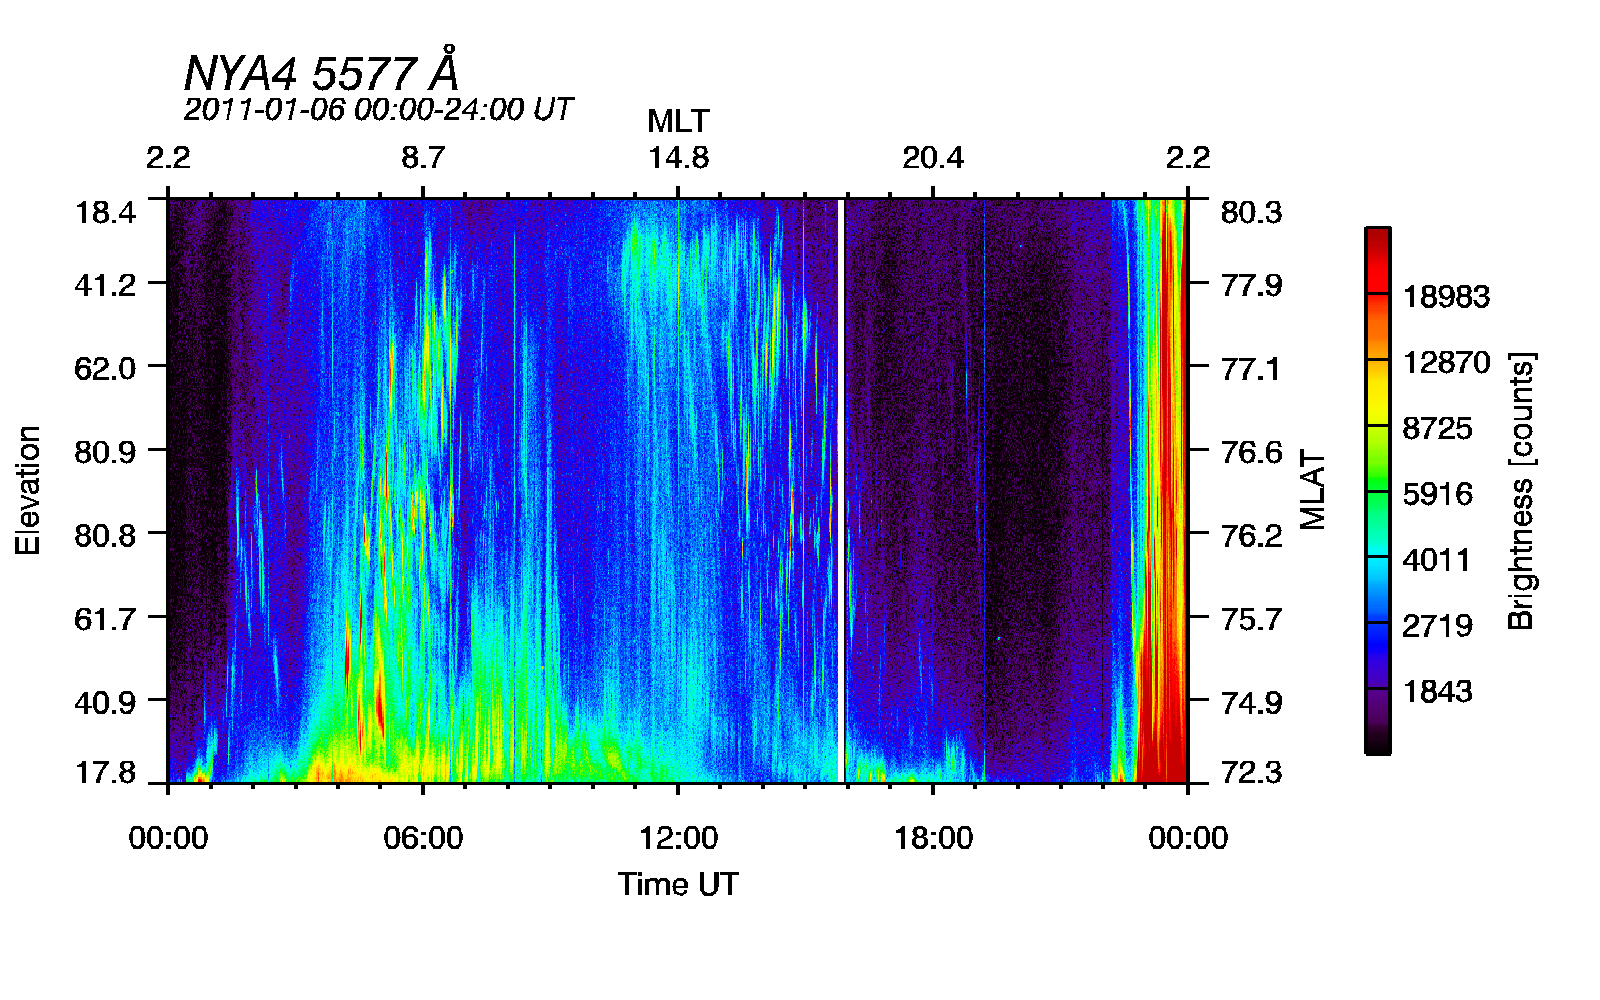
\includegraphics[scale = 0.20]{am-0024-5577.png}
	\centering
	\caption{Keogram of the All-Sky camera}
	\label{a1}
\end{figure}

\subsection{ACE}

The Advanced Composition Explorer, short ACE, is a satellite from NASA, which is among other things used to study the solar wind and its magnetic field. It orbits around the sun at the Lagrangian point $L_1$ so that it is always at a stable region between the earth and the sun, about $1.5 \cdot 10^6 km$ away from earth. 
One instrument of the satellite we are going to use is the SWEPAM (Solar Wind Electron, Proton and Alpha Monitor). With the instrument we can analysize the solar wind bulk speed to determine how much time it will need from the satellite to the earth. 
The other instrument we will use is the MAG (Magnetometer) to study the magnetic field of the solar wind.


\subsection{SuperDARN}

SuperDARN (Super Dual Auroral Radar Network) is a network of radars that consists of more than 30 low-power high frequency radars. It is used to measure plasma convection in the F-Region of the ionosphere at a high latitude. In figure \ref{s1} the area the radars of SuperDARN cover is shown. It can be seen that nearly the whole northern polar cap is covered by the radars. On Russia's side some ground at high latitude is not covered by the radars.
The radars are using the Doppler effect to measure convection. They send out electromagnetic waves at a specific frequency. In the Ionosphere the waves get reflected and have a Doppler shift due to movement of the plasma. From the change in frequency of the waves which return to the instruments, the velocity of the plasma can be determined.

\begin{figure}[h]
	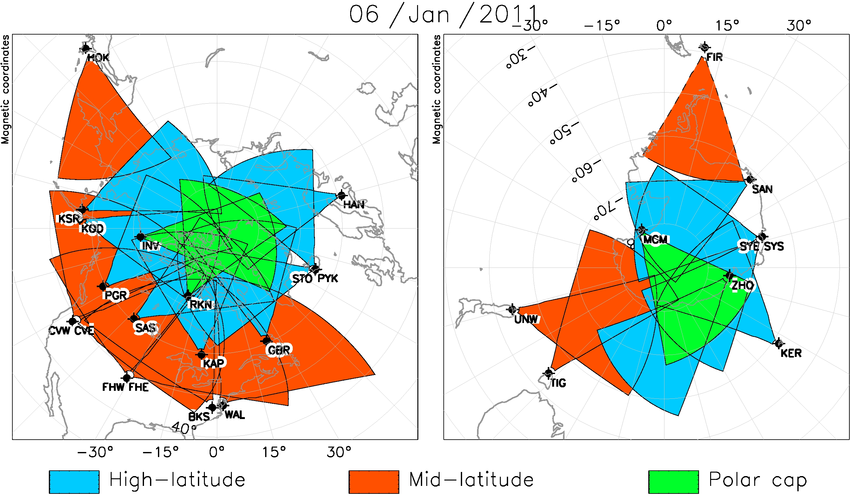
\includegraphics[scale = 1.5]{sd_1.png}
	\centering
	\caption{Covered area of the SuperDARN}
	\label{s1}
\end{figure}

\subsection{AMPERE}

AMPERE stands for "Active Magnetosphere and Planetary Electrodynamics Response Experiment". It uses the over 60  Iridium satellites which are orbiting earth to get information about the space weather. On the satellites are magnetometers to measure magnetic fields. From the measurement of those fields, field-aligned currents can be derived, using Amperes law. Thus the currents drawn in the diagrams belonging to AMPERE are not measured directly. Because of the amount of iridium satellites, the measurements are always covering the whole earth.

\subsection{Ground-based magnetometers}

In this project we are going to analyse the data on Ground-based magnetometers. Most of the magnetometers we are using are located in Norway, Sweden or Finland. A current always generates a magnetic field (Ampere's law). Hence by measuring the magnetic field on the ground, currents in the Ionosphere can be measured indirectly.

\section{Observations}

\subsection{All-Sky Camera}

The figure \ref{fig:sfig1} and \ref{fig:sfig2} show the keograms of the All-Sky Camera for the whole day on the 06.01.2011 for the green and red aurora. We look at the time span from 18 to 24 UT. On the first sight it can be seen, that before 22 UT there is nearly no aurora, while after 22 UT there is a big onset of aurora. This timespan, 22-24 UT, will be discussed the most in this section.

Between 18 UT and 19 UT (figure \ref{fig:sfig3} and \ref{fig:sfig4}) it can be seen, that the camera detects a lot of light at low latitudes. Most of this bright structure is outside of the range of the imager and is very stable in time. At 18:45 UT there is a bright source at higher latitude, which moves southward for 10 minutes. By looking at the pictures the camera took separately and comparing the structure at both wavelengths, it can be seen that this is probably a cloud, which moves southward and then dissolves. 
In the timespan 19-22 UT, no auroral activity is happening in the area the All-sky camera observes. It could be, that due to dayside reconnection the polar cap expanded in size, such that auroras can only happen at latitudes lower than the ones observable for the camera.

 In figure \ref{fig:sfig5}, \ref{fig:sfig6} and \ref{i1} it can be seen, that, starting with 22:20 UT, a long aurora forms at the western sky up to 82° geomagnetic latitude and moves southward down to 75° MLAT at 22:50 UT. During the end of that movement, starting from 22:45 UT, there is a large onset of aurora, which starts at low latitudes (72.3 MLAT). This onset then moves very quickly to higher latitudes. At 23:28 the auroras are already at 80° MLAT and stay at latitudes this high up until 0:00 UT. During that movement, the auroras a very unstable in position and brightness, for example when they increase their intensity a lot at 23:10 UT, then get less intense and peak again from 23:25 to 23:33 UT. The last peak of onset of auroras then is from 23:50 to after 0:00 UT.
 Also, starting from 22:10 auroras at low latitudes around 70° MLAT can be seen(figure \ref{i1}). Those auroras are the ones, that brighten at the big onset of aurora at 22:45 UT.
The biggest onset of green aurora is between 23:28 and 23:29 UT. In this time frame the green aurora covers nearly the whole sky, while the red is not as strong. The red aurora is especially strong between 23:03 and 23:09 UT.
The sudden strong increases of auroral activity starting from 22:45 UT are a sign of a starting expansion phase of a substorm.

 In the night of the 06.01.2011 it looks like there is a especially big substorm happening between 22:20 and 24:00 UT. At 22:45 the expansion phase of this substorm starts. It has the typical characteristics of this phase, because the aurora suddenly brightens, moves poleward quickly and then already fills nearly the whole sky at 23:28 UT (figure \ref{i2}). In this phase, the auroras move from 70° MLAT at 22:40 UT to 81°-82.5° MLAT at 23:32 UT and stay at this latitude to after 24:00 UT. The start of an expansion phase is due to sudden nightside reconnection at the near-earth neutral-line, which has has distance of $20 R_E-30 R_E$ to earth.
 
 It happens that the intensity of auroral activity decreases between 23:05 and 23:20 UT and 23:45 and 23:50 UT, but we would not describe this time-spans as a recovery phase, because they last a very short time and are quickly followed by a big increase of auroral activity again. The real recovery phase of the substorm begins after 24:00 UT.   

\begin{figure}[h]
	\begin{subfigure}{.5\textwidth}
		\centering
		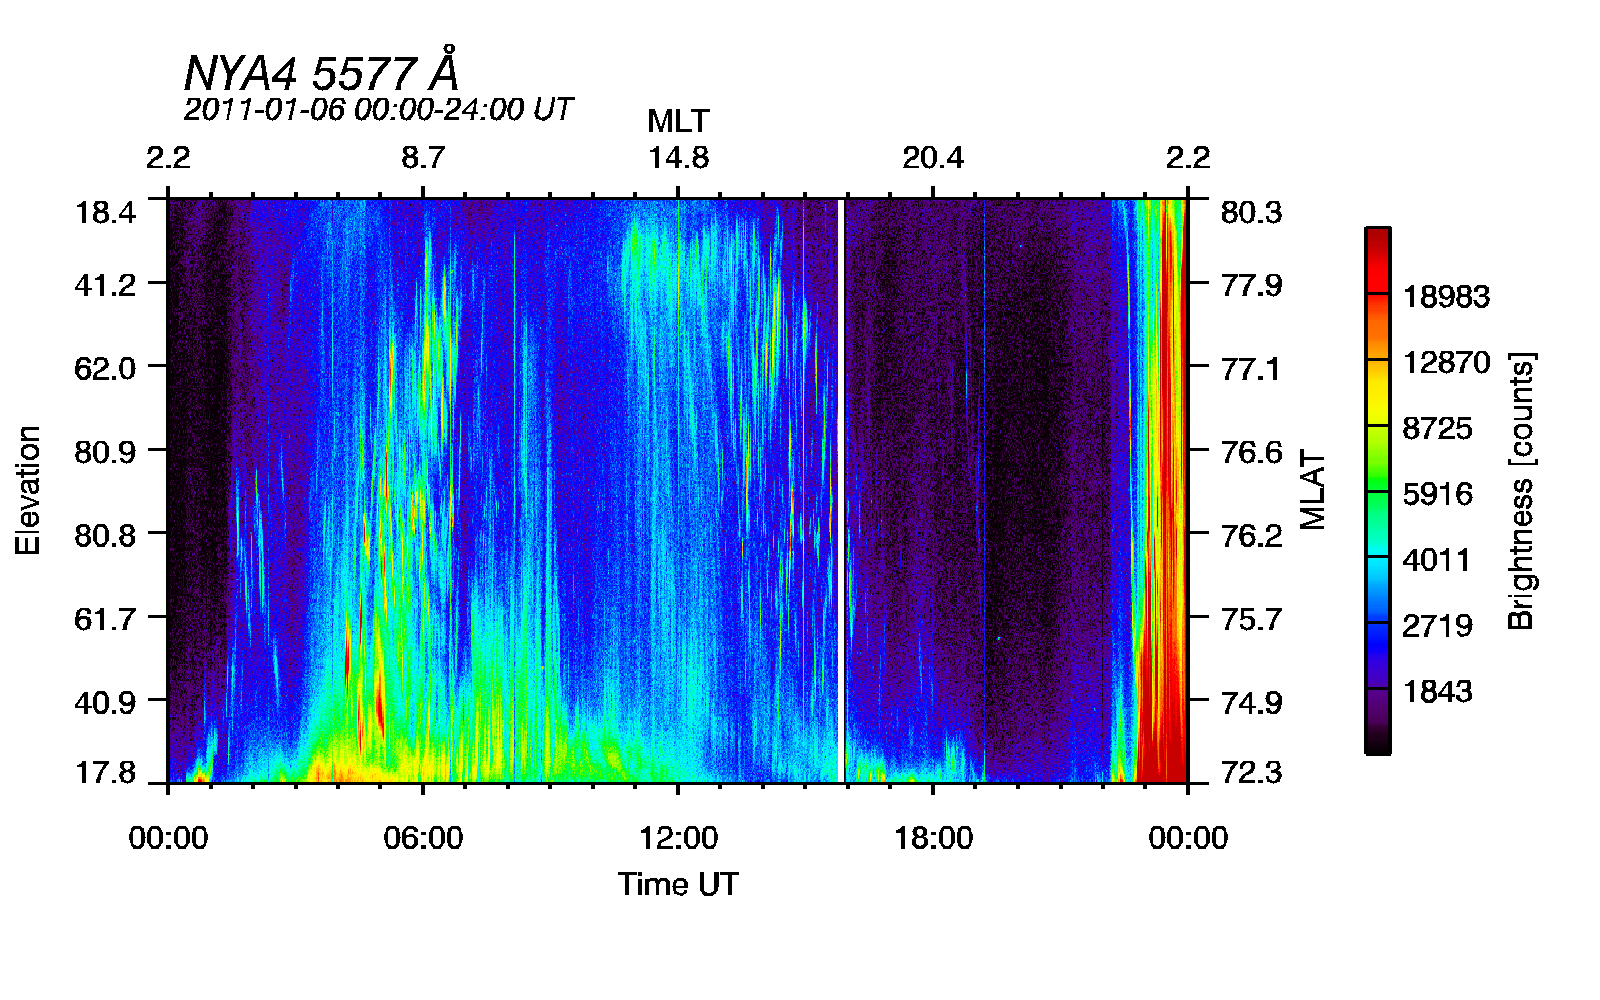
\includegraphics[width=.8\linewidth]{am-0024-5577.png}
		\caption{0-24 UT, 5577 Å}
		\label{fig:sfig1}
	\end{subfigure}
	\begin{subfigure}{.5\textwidth}
		\centering
		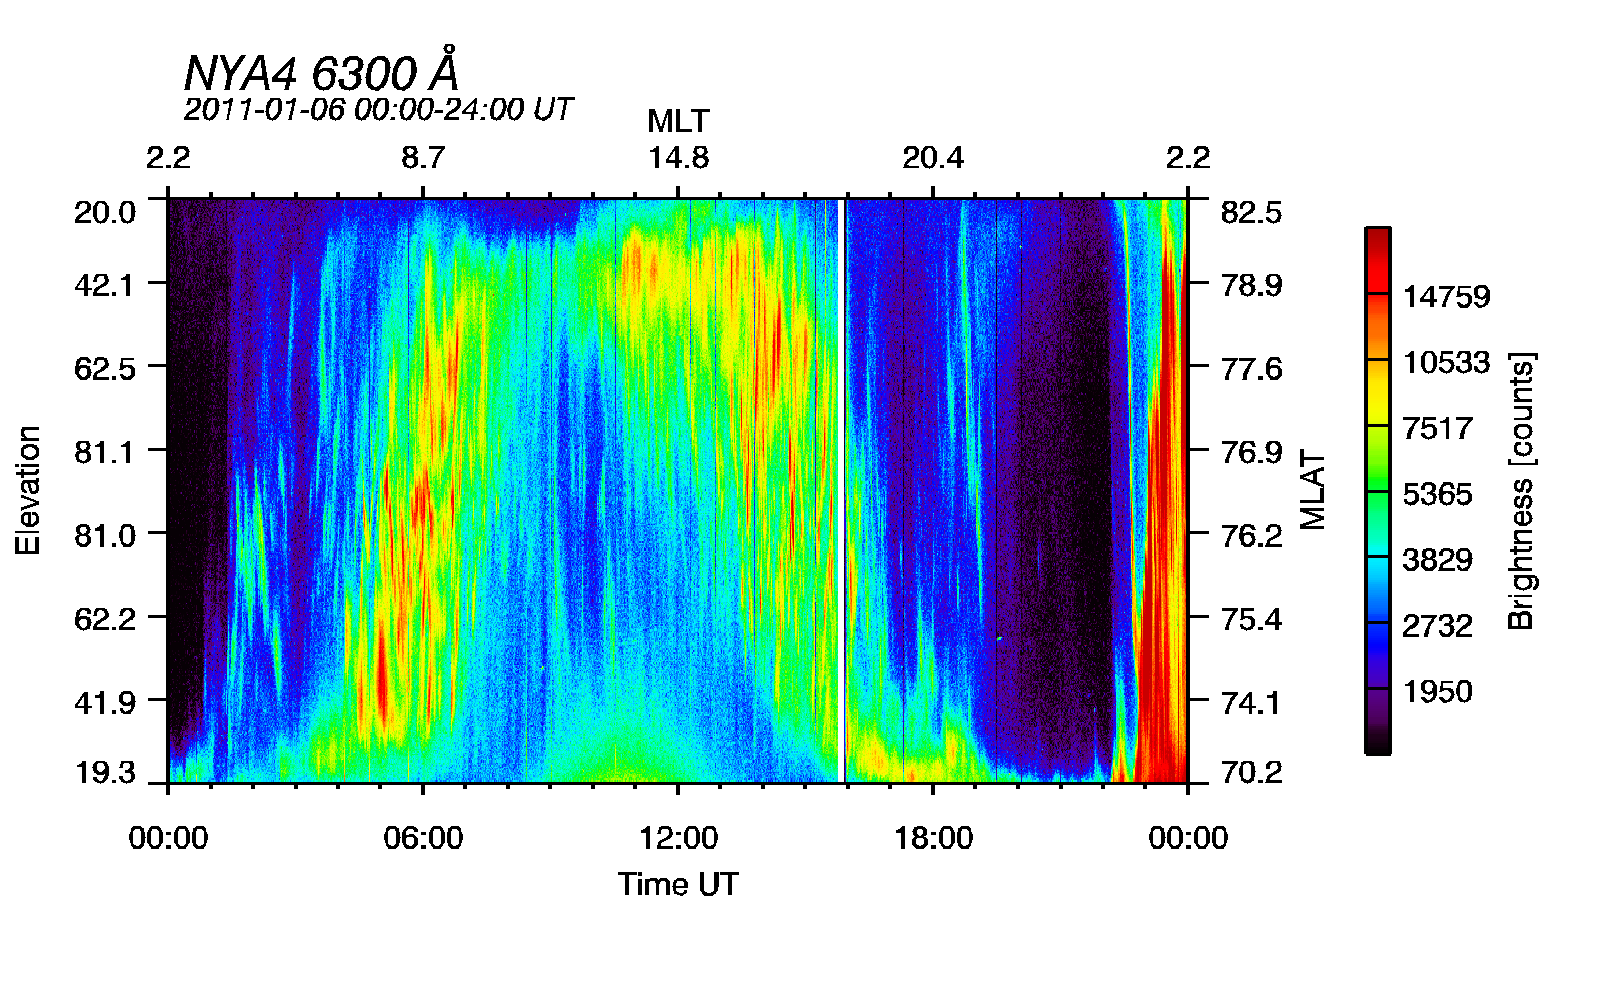
\includegraphics[width=.8\linewidth]{am-0024-6300.png}
		\caption{0-24 UT, 6300 Å}
		\label{fig:sfig2}
	\end{subfigure}
	\begin{subfigure}{.5\textwidth}
		\centering
		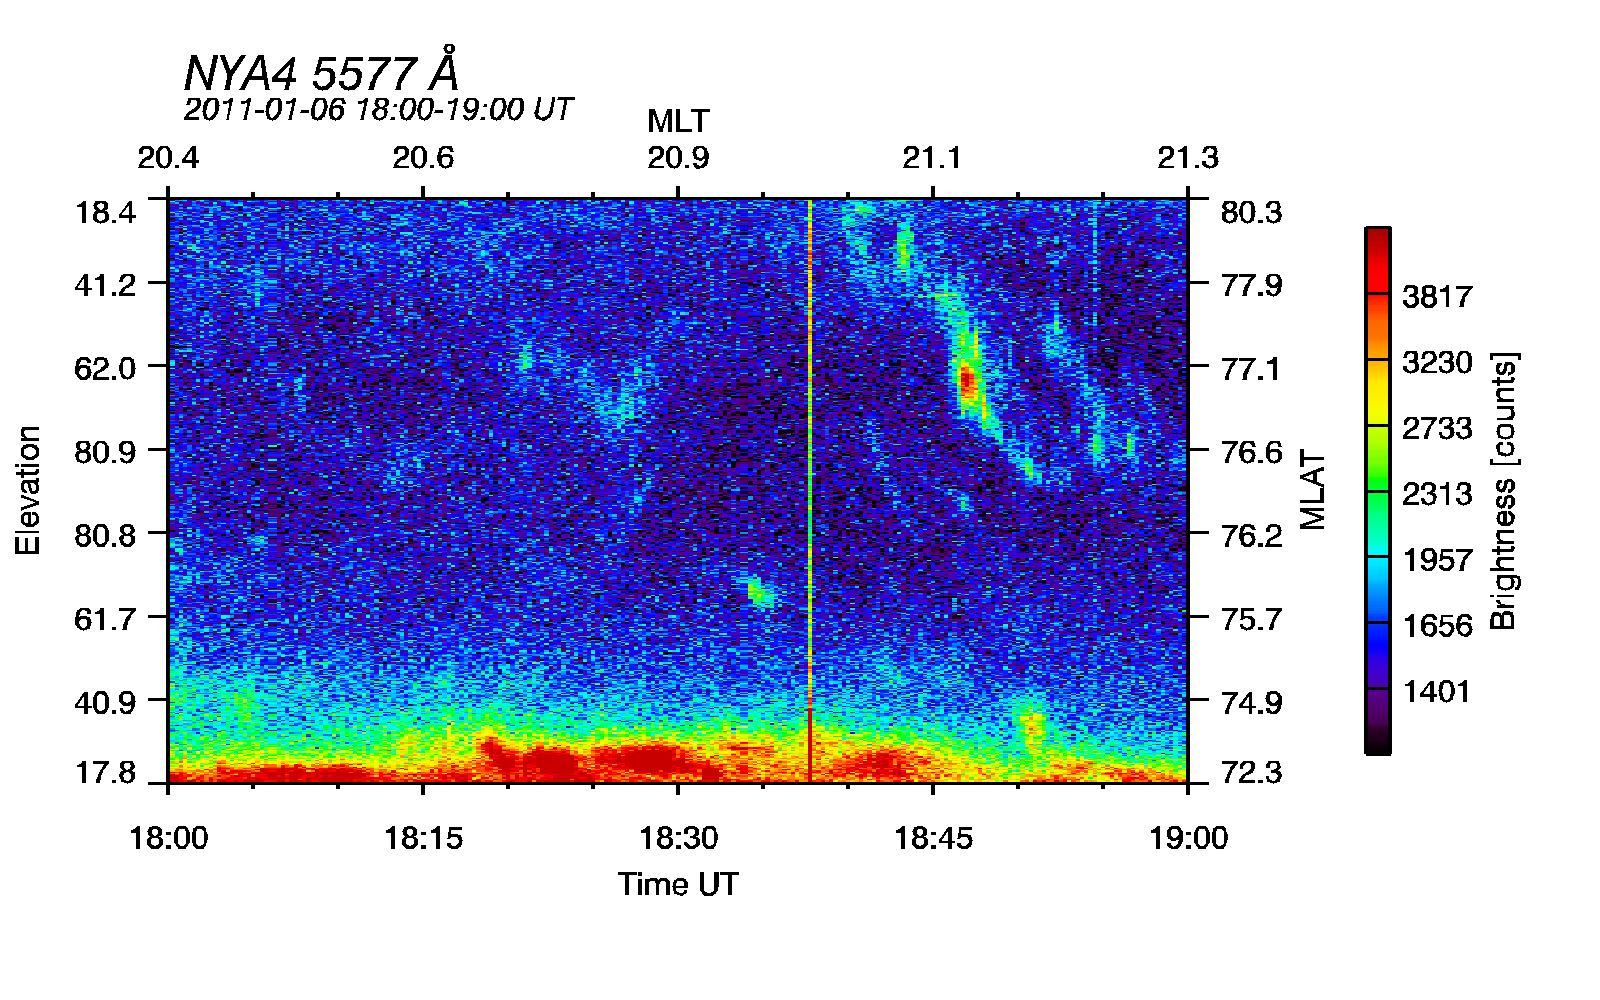
\includegraphics[width=.8\linewidth]{am-1819-5577.png}
		\caption{18-19 UT, 5577 Å}
		\label{fig:sfig3}
	\end{subfigure}
	\begin{subfigure}{.5\textwidth}
		\centering
		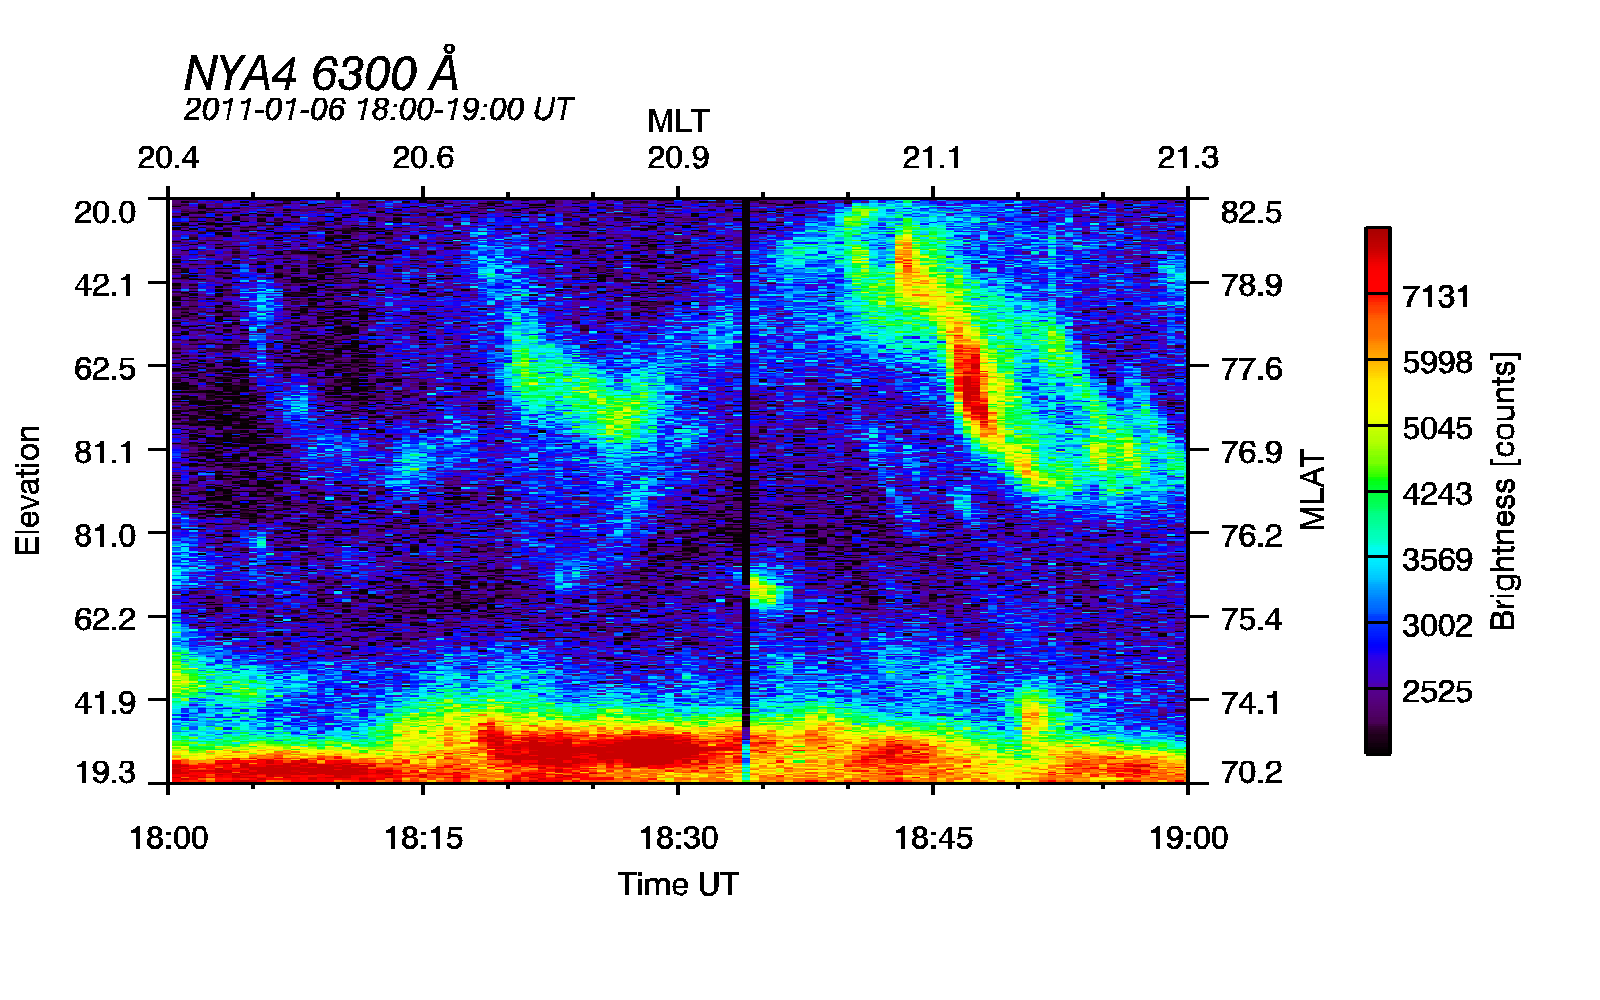
\includegraphics[width=.8\linewidth]{am-1819-6300.png}
		\caption{18-19 UT, 6300 Å}
		\label{fig:sfig4}
	\end{subfigure}
	\begin{subfigure}{.5\textwidth}
		\centering
		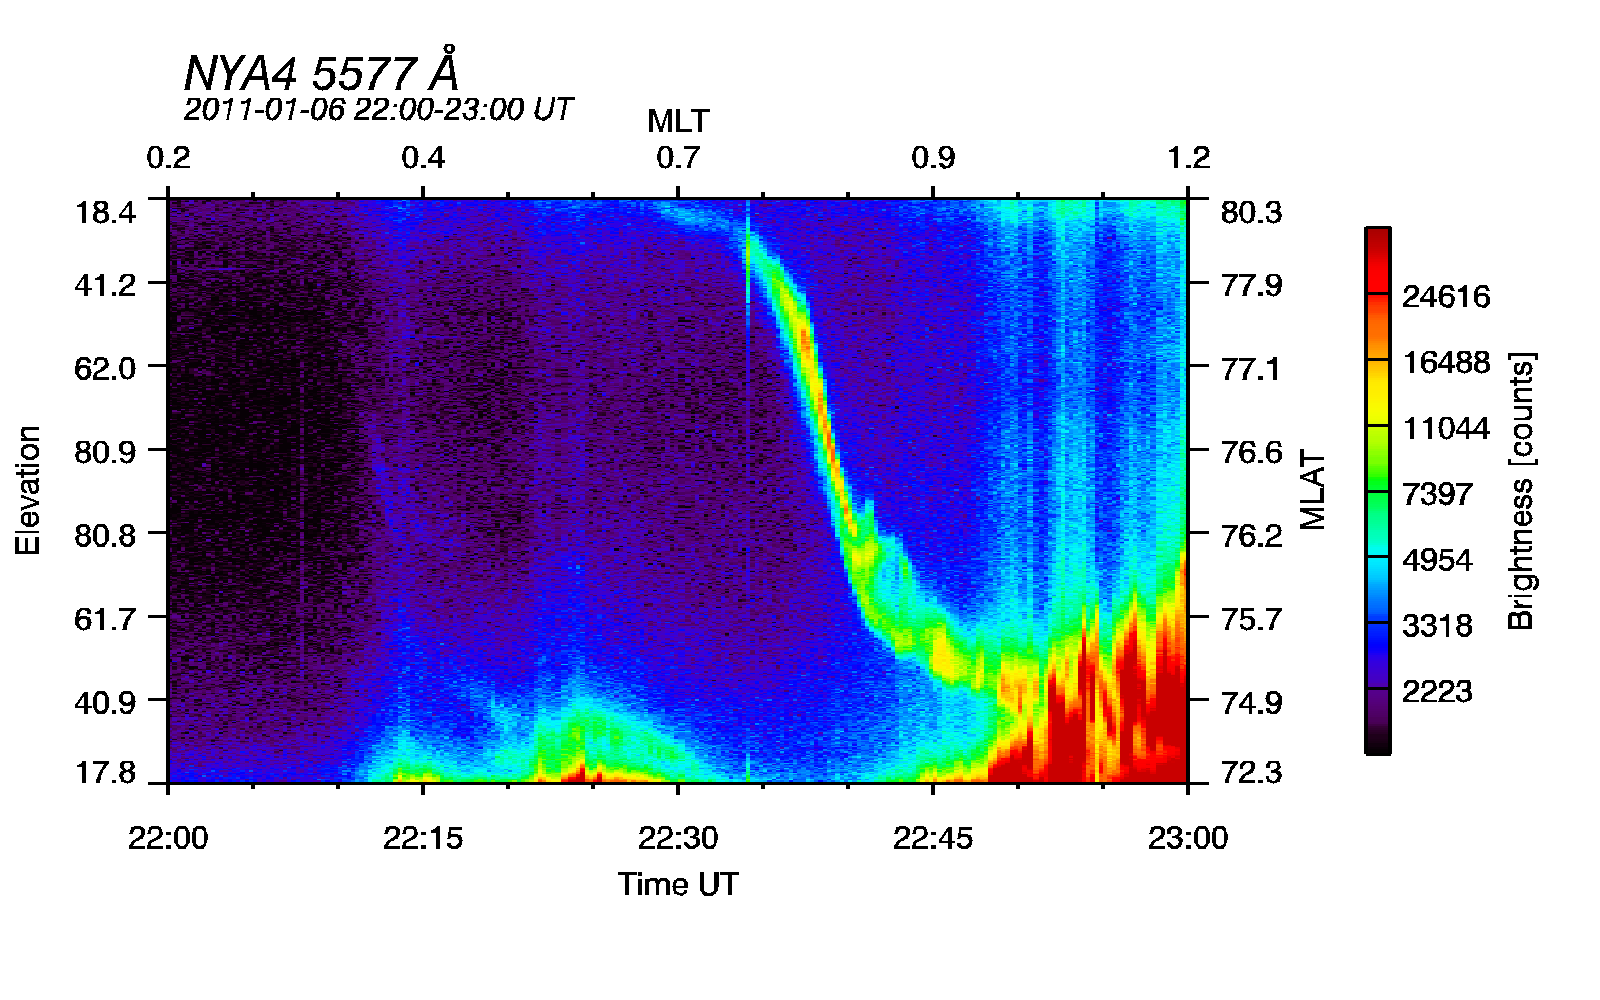
\includegraphics[width=.8\linewidth]{am-2223-5577.png}
		\caption{22-23 UT, 5577 Å}
		\label{fig:sfig5}
	\end{subfigure}
	\begin{subfigure}{.5\textwidth}
		\centering
		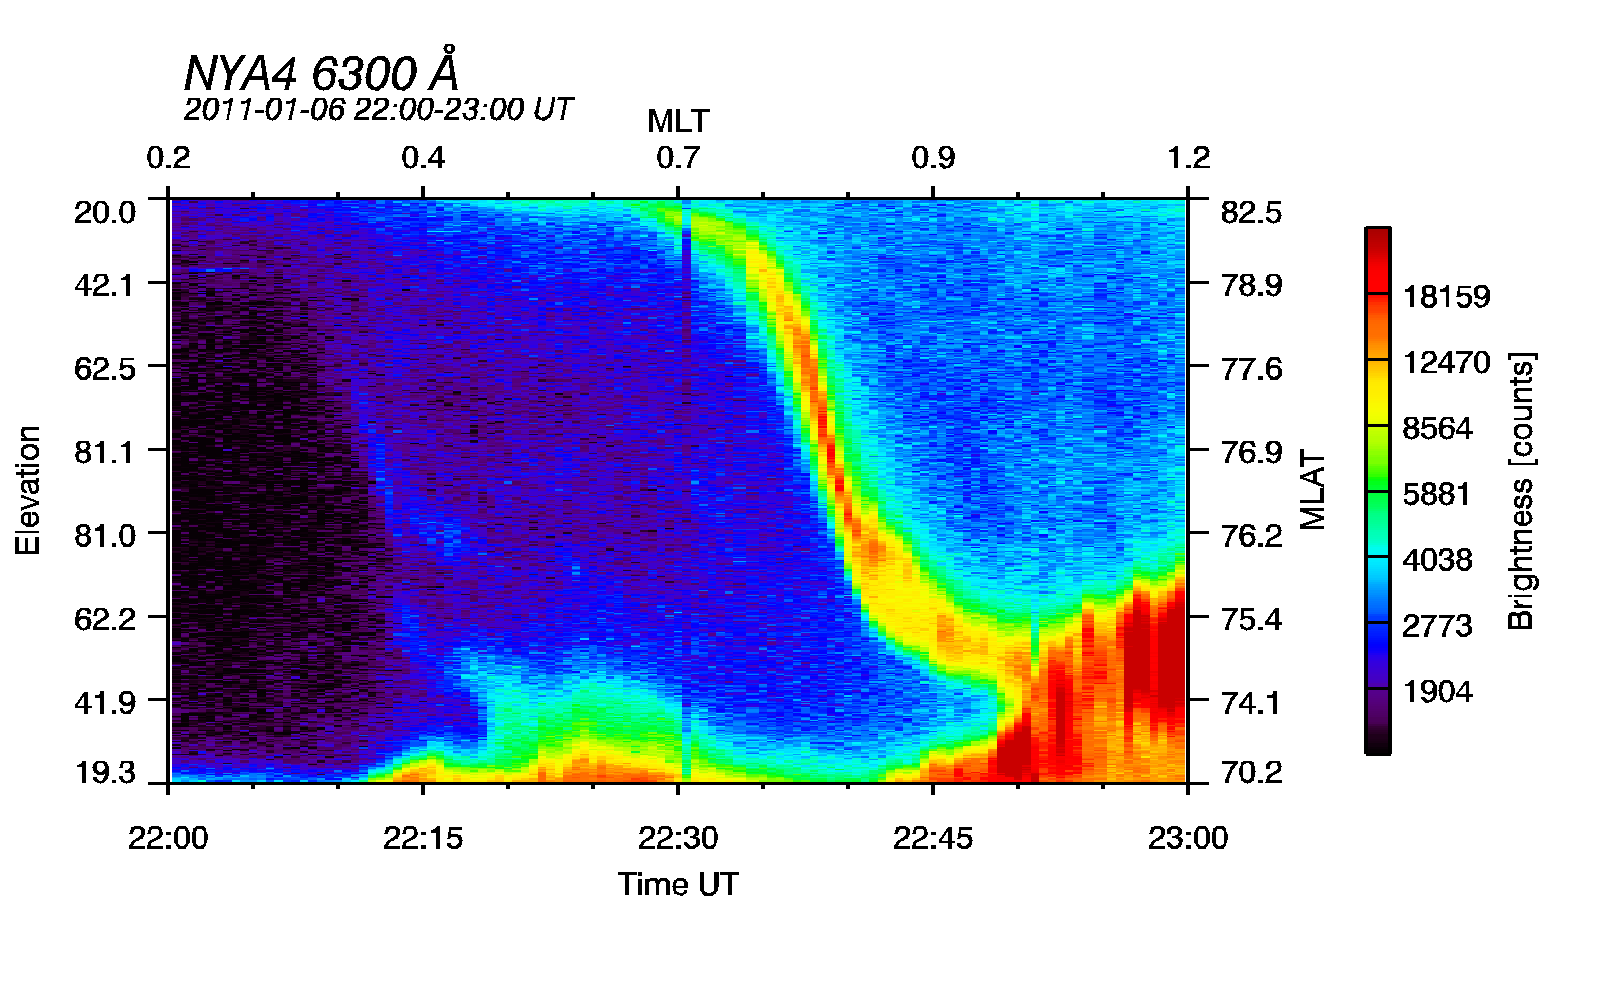
\includegraphics[width=.8\linewidth]{am-2223-6300.png}
		\caption{22-23 UT, 6300 Å}
		\label{fig:sfig6}
	\end{subfigure}
	\begin{subfigure}{.5\textwidth}
		\centering
		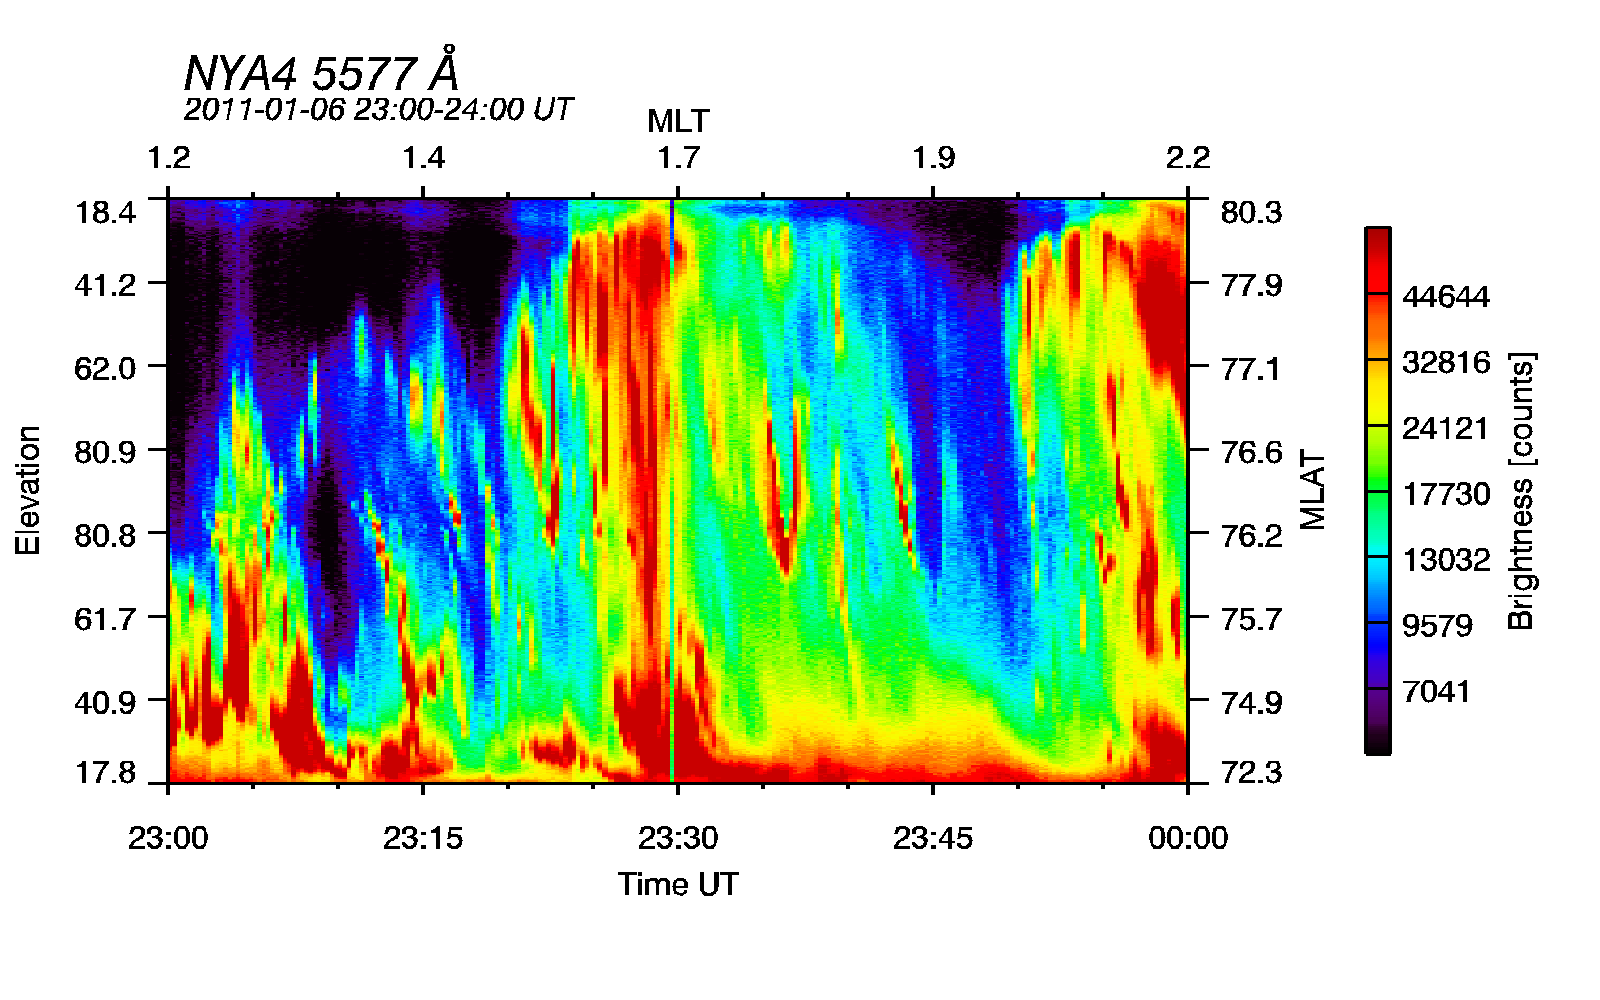
\includegraphics[width=.8\linewidth]{am-2324-5577.png}
		\caption{23-24 UT, 5577 Å}
		\label{fig:sfig7}
	\end{subfigure}
	\begin{subfigure}{.5\textwidth}
		\centering
		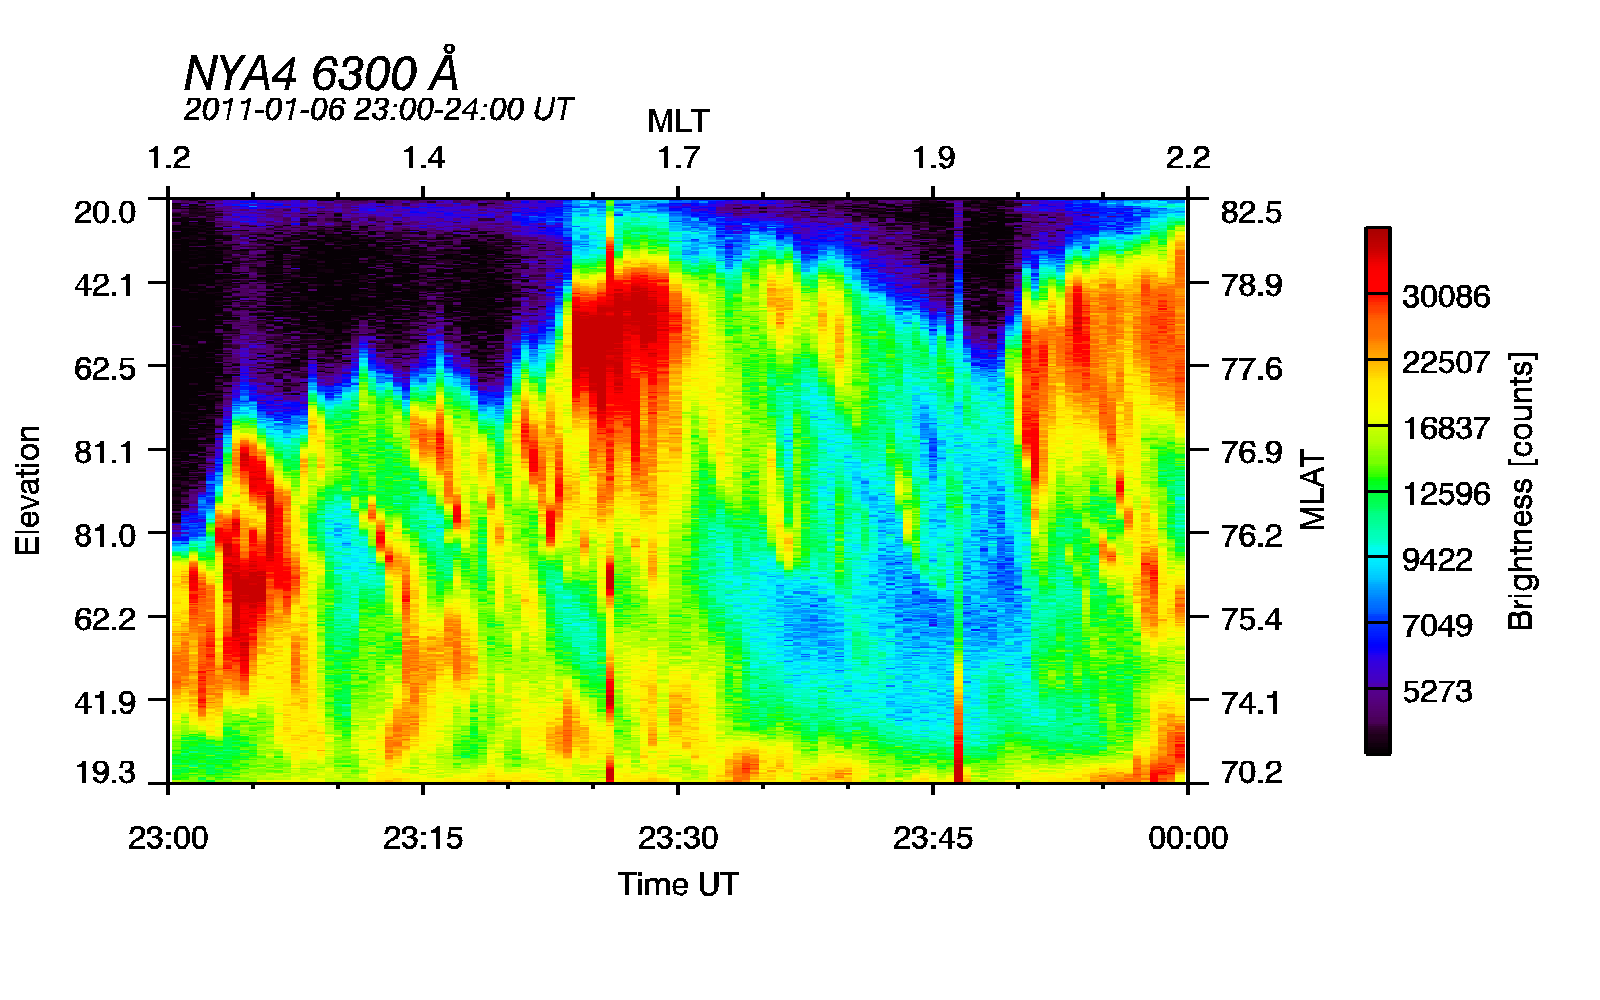
\includegraphics[width=.8\linewidth]{am-2324-6300.png}
		\caption{23-24 UT, 6300 Å}
		\label{fig:sfig8}
	\end{subfigure}
	\caption{Keograms of the All-sky camera for different times and wavelengths }
	\label{fig:fig}
\end{figure}

\begin{figure}
\begin{subfigure}{.5\textwidth}
	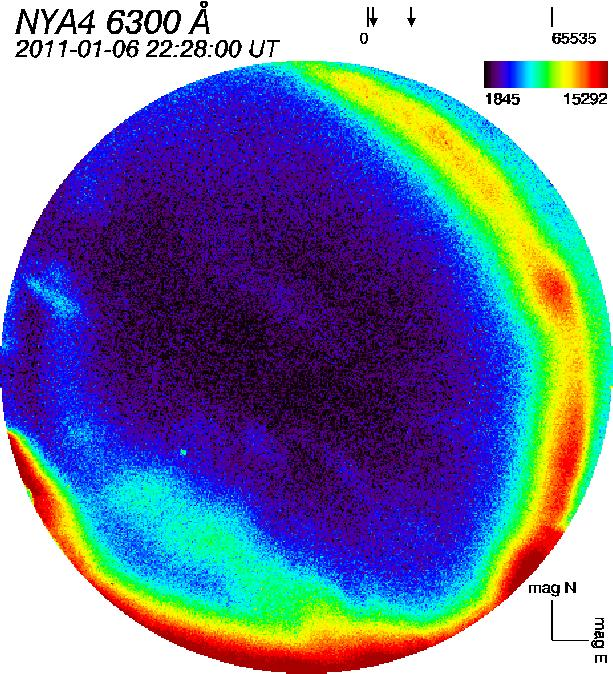
\includegraphics[width=.8\linewidth]{ame-2228-6300.jpg}
	\centering
	\caption{22:28 UT, $\lambda$ = 6300 Å}
	\label{i1}
\end{subfigure}
\begin{subfigure}{.5\textwidth}
	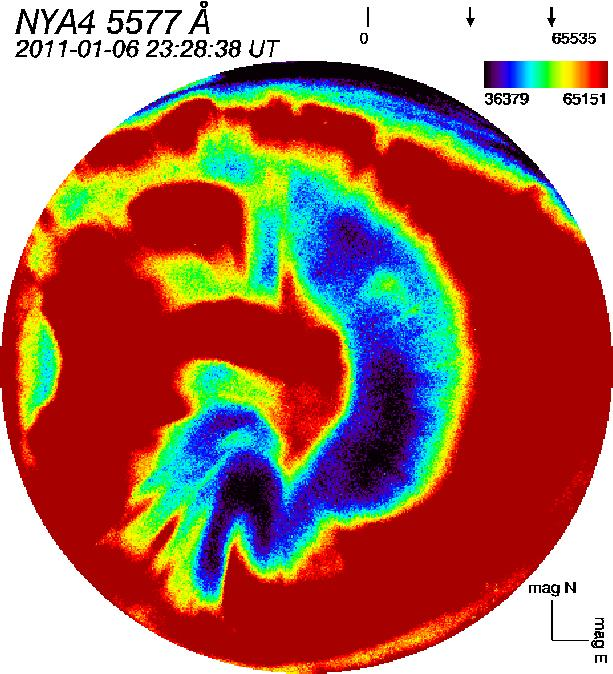
\includegraphics[width=.8\linewidth]{ame-2328-5577.jpg}
	\centering
	\caption{23:28 UT, $\lambda$ = 5577 Å}
	\label{i2}
\end{subfigure}
\caption{Images of the All-sky camera}
\end{figure}


\subsection{ACE}

I figure \ref{ace1} the components of the magnetic field of the solar wind can be seen in the timespan 17:00-23:10 UT. In the coordinate system, we are using, the geocentric solar magnetospheric system (GSM), it only depends on the z-component of the magnetic field, if magnetic reconnection at the magnetopause is possible. Is the z-component of the magnetic field of the solar wind lower than zero, it has the opposite sign than the terrestrial magnetic field. Thus magnetic reconnection is possible. 

It can be observed, that between 17:00 and 20:10 UT, most of the time $B_Z$ is bigger than zero. Hence, nearly all this time magnetic reconnection is not possible at the magnetopause.
At 20:10 UT $B_Z$ drops more than $20 nT$ and then stays negative nearly all the time until the end of our observed time span. Just at 22:00 UT and around 21:20 UT it goes positive for a very short amount of time. Thus from the time, the solar wind, which passes the ACE at 20:10 UT, reaches the earth, magnetic reconnection is possible. 

In our coordinate system, the x-axis is parallel to the connection line of earth and sun. Because the satellite is between those two objects, we only need to look at the solar wind velocity in x-direction to calculate, how long the wind needs from the satellite to earth.
In the timespan 17:00-20:00 UT the velocity $v_x$ of the solar wind is nearly constant at $v_x = 350 \frac{km}{s}$ (figure \ref{ace3}). In this time the distance between satellite and earth, $s_x$, is between $1,4509 \cdot 10^6 km$ and $1,4512 \cdot 10^6 km$. Thus the solar wind needs approximately $t = \frac{1,4510 \cdot 10^6 km}{350 \frac{km}{s}} = 69 min$ to the earth.

At 20:10 UT, when the magnetic field $B_Z$ of the solar wind gets negative, the solar wind has a velocity of $(370 \pm 10) \frac{km}{s}$ and the distance between satellite and earth is $(1.4513 \pm 0.0001) \cdot 10^6 km$. With this values, we can calculate the time, the solar wind from 20:10 needs to reach the earth. We use the approximation, that the solar wind stays at the same velocity between earth and satellite. The time the wind needs is $t = \frac{1.4513 \cdot 10^6 km}{370 \frac{km}{s}} = 65 min$. Thus it needs $65 \pm 2 min$ from the satellite to earth and arrives at the earth at $21:13 UT - 21:17 UT$. From this time, magnetic reconnection can happen at the magnetopause.


\begin{figure}[h]
	\begin{subfigure}[h]{.5\textwidth}
		\centering
		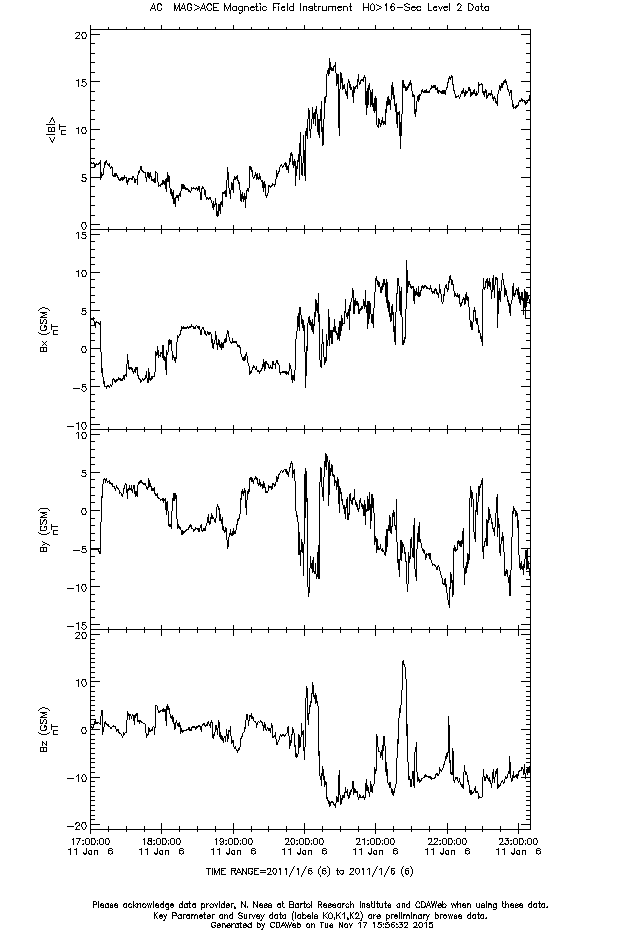
\includegraphics[width=.8\linewidth]{ace-17-2310-b.png}
		\caption{Magnetic field of the solar wind, 17:00-23:10 UT}
		\label{ace1}
	\end{subfigure}
	\begin{subfigure}[h]{.5\textwidth}
		\centering
		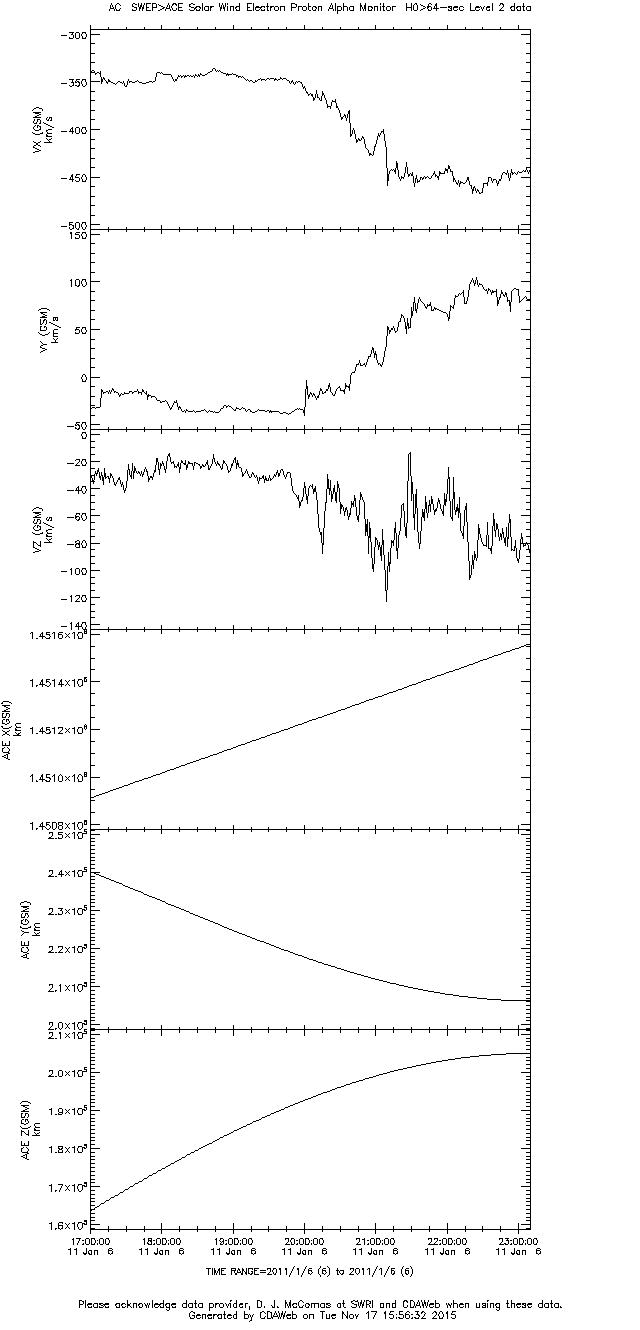
\includegraphics[width=.8\linewidth]{ace-17-2310-v-s.png}
		\caption{Velocity of the solar wind and position of the satellite, 17:00-23:10 UT}
		\label{ace3}
	\end{subfigure}
	\caption{Measurements of the ACE (GSM coordinate system)}
	\label{ace}
\end{figure}


\subsection{AMPERE}

The figures of AMPERE show basically the magnetic field on Earth, resulting in a field aligned current density,  and this field is measured by satellites, where in the plot, for instance, if the field vectors point in a certain direction, the tail refers to the satellite position.
For the current density, choosing the North pole, we can see an pattern where the currents encircle the pole. Its intensity is represented by the intensity in the colors. The colors red and blue represent the direction of these currents, where:


Red – Upward currents;
Blue – Downward currents.


These field-aligned currents are called Birkeland currents and should follow a certain pattern, where at the dawn and poleward, the currents must be down into the ionosphere, and upward-currents at the dusk. Now we must analyse the behaviour of these fields and currents for each time interval. For each hour, we plot values which will help us to see when the aurora starts to happen with respect to these parameters.


18-19 UT (figure \ref{amp1}): Between 18:00 UT-18:10 UT, occurs the highest magnetic activity in this period. After that, the current density is narrow, and no significant phenomena for our case is suggested.


19-20 UT (figure \ref{amp2}): The current density remains narrow with a short increase at 19:30 UT, but nothing more. These results agree with the IMF data, where we see, that in this time period no interaction between IMF and terrestrial magnetic field is possible. What we expect is, that after 21 UT, the pattern will change due to the change of sign of the $B_Z$ of the IMF.


20-21 UT (figure \ref{amp3}): Around 20:10 UT, and also 20:50 UT, B gets slightly more intense, so as the current density, but just at 21 UT, there is a significant increase in activity, comparing to previous times.


21-22 UT (figure \ref{amp4}): The slight increase at 21 UT of the current density gets bigger 10 minutes after, but in the interval 21:20 UT-21:40 UT, decreases again. But, at 21:50 UT, the current density suddenly gets bigger considerably.


According to data from ACE, the solar wind with negative $B_Z$ arrives Earth between 21:13 UT-21:17 UT. From this time on, magnetic reconnection can happen at the magnetopause. This time is basically when due to the negative  $B_z$-component of the incoming solar wind, magnetic reconnection at the dayside is possible. The All-sky Camera states that the auroral activity starts around 22:20 UT, so magnetic reconnection has already happened, so we must look again to the data between 21:50 UT and 22:20 UT on the current density plot.


22-23 UT (figure \ref{amp5}): This increase continues approximately linear until 22:10 UT, where the current density becomes intense, mostly around the area of Greenland, Norway and Russia. At 22:50 UT, the currents become more distributed.


23-24 UT (figure \ref{amp6}): The magnetic activity becomes highly intense from now on, with the current well distributed, around the North pole, and so the B vectors have their peak of magnitude, especially from, 23:20 UT and, this happens also in the Svalbard area, where the other data we are analysing comes from.

\begin{figure}[h]
	\begin{subfigure}[h]{.5\textwidth}
		\centering
		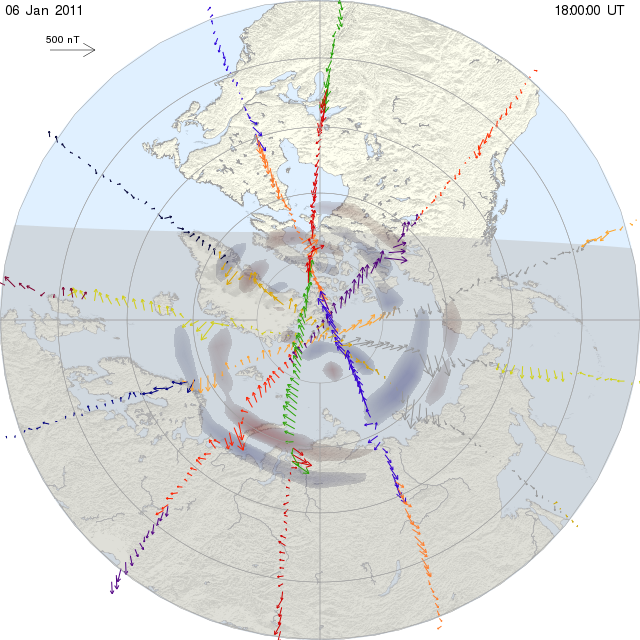
\includegraphics[width=.8\linewidth]{1294336800north.png}
		\caption{Magnetic field and currents at the northern polar cap, 18:00 UT}
		\label{amp1}
	\end{subfigure}
	\begin{subfigure}[h]{.5\textwidth}
		\centering
		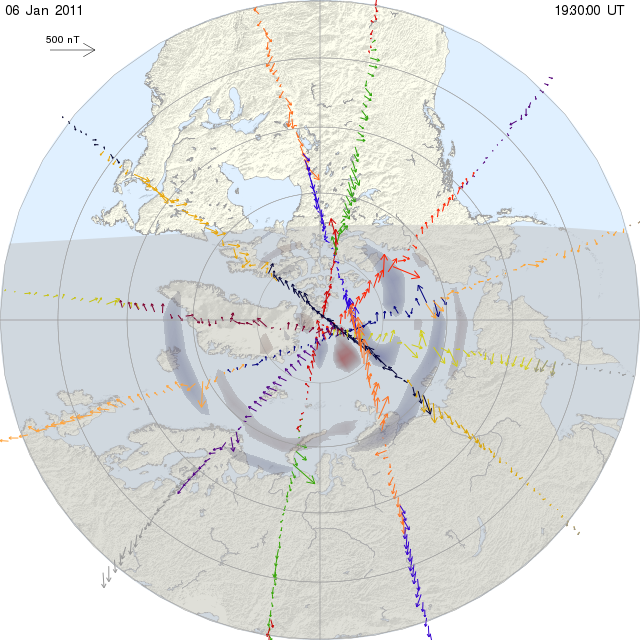
\includegraphics[width=.8\linewidth]{1294342200north.png}
		\caption{Magnetic field and currents at the northern polar cap, 19:30 UT}
		\label{amp2}
	\end{subfigure}
	\begin{subfigure}[h]{.5\textwidth}
		\centering
		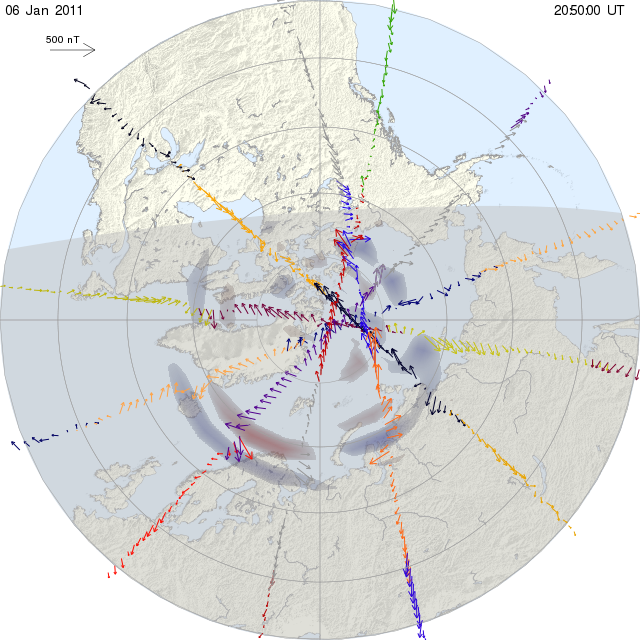
\includegraphics[width=.8\linewidth]{1294347000north.png}
		\caption{Magnetic field and currents at the northern polar cap, 20:50 UT}
		\label{amp3}
	\end{subfigure}
	\begin{subfigure}[h]{.5\textwidth}
		\centering
		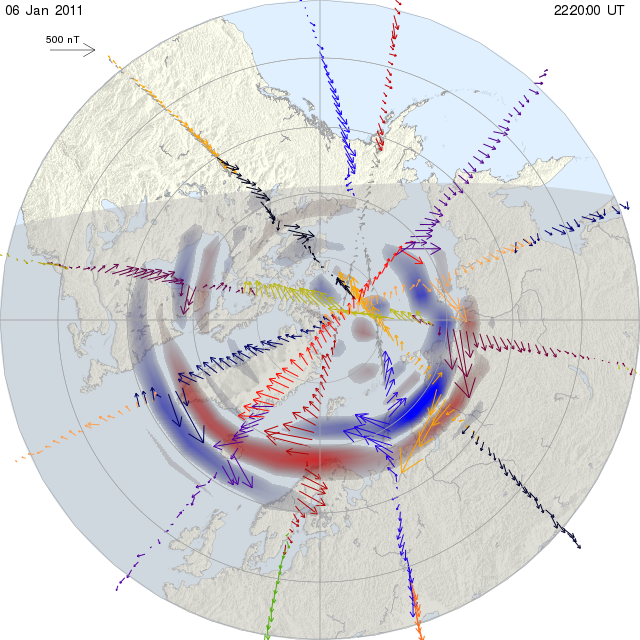
\includegraphics[width=.8\linewidth]{1294352400north.png}
		\caption{Magnetic field and currents at the northern polar cap, 22:20 UT}
		\label{amp4}
	\end{subfigure}
	\caption{Measurements of AMPERE}
	\label{amp}
\end{figure}
\begin{figure}[h]
	\begin{subfigure}[h]{.5\textwidth}
		\centering
		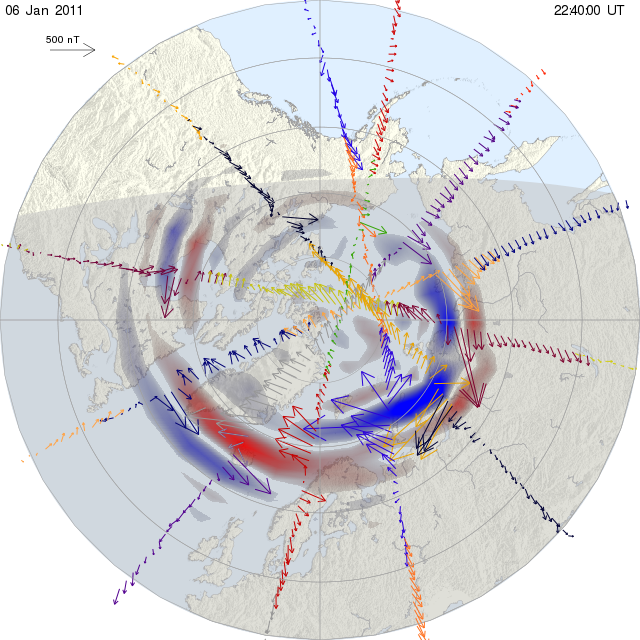
\includegraphics[width=.8\linewidth]{1294353600north.png}
		\caption{Magnetic field and currents at the northern polar cap, 22:40 UT}
		\label{amp5}
	\end{subfigure}
	\begin{subfigure}[h]{.5\textwidth}
		\centering
		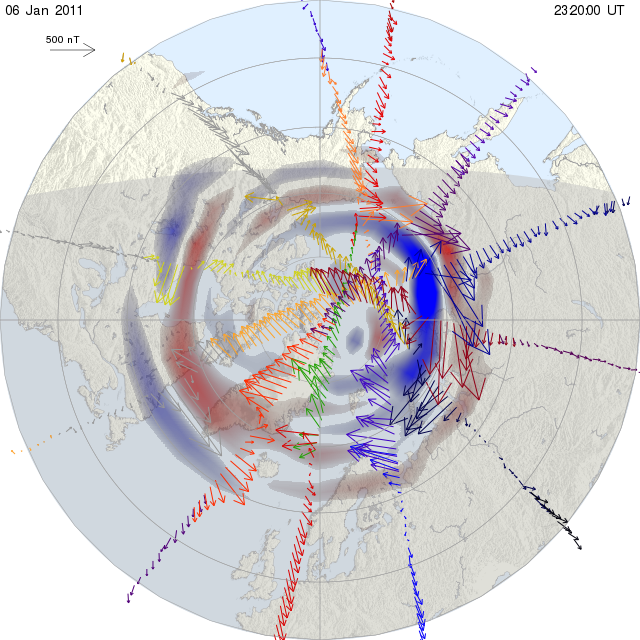
\includegraphics[width=.8\linewidth]{1294356000north.png}
		\caption{Magnetic field and currents at the northern polar cap, 23:20 UT}
		\label{amp6}
	\end{subfigure}
	\newpage
	\begin{subfigure}[h]{.5\textwidth}
		\centering
		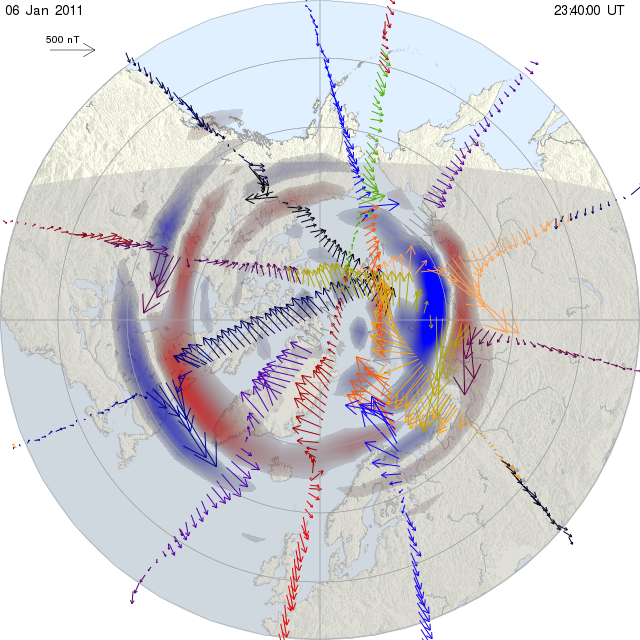
\includegraphics[width=.8\linewidth]{1294357200north.png}
		\caption{Magnetic field and currents at the northern polar cap, 23:40 UT}
		\label{amp7}
	\end{subfigure}
	\caption{Measurements of AMPERE}
	\label{ampp}
\end{figure}

\subsection{Ground-Based Magnetometers}

Looking at the z-component of B, it is possible to check the field in the Earth. We look at the magnetic field at different locations. One of those is the Ny Ålesund station, represented by NAL. At figure \ref{mag1} we choose the time interval 18 UT-24 UT. At 18:00 UT-22:10 UT magnetic activity starts to increase. There is an even bigger increase around 22:40 UT, peaking at 23 UT, with just a local minimum at 23:30 UT and increasing again in a short period of time, until 24:00 UT. Looking now on the plot in more detail, lets see hat happens in each hour, in the mentioned interval:

Between 18 and 19 UT (figure \ref{mag2}), the field oscillates on maximum values of $10 nT$, and keeping  approximately constant value for few minutes, which is not enough to have reconnection, if the IMF  is present.

Between 19 UT-20 UT (figure \ref{mag3}), there is more oscillation in the field, but at even smaller values, where we can see that the scale gets smaller, from $20 nT$ to $10 nT$.
From 20 UT to 21 UT (figure \ref{mag4}), the behaviour is quite similar to the first interval, but with low peaks of magnitude. However, in this time interval, we calculated that around 20:10 UT, the solar wind IMF with negative $B_Z$ hits the ACE satellite, and in about one hour, would arrive at the magnetopause, so we should expect some activity in the next hour.

Now we have more magnetic activity for a longer time (figure \ref{mag5}), especially in the interval between 21.35 UT-21:45 UT. But as we can see from the All-sky Camera and because of the decrease in magnitude after this period, magnetic reconnection at the nightside still does not happen to a bigger extent. But looking at the time that the field values start to increase, apparently agrees with the computation of time, when the negative $B_Z$ component of the IMF reaches the earth, which is around 21:17 UT. From this time the measured field, using the Ground-Based Magnetometers, increases (almost) continuously.

At the next time interval (figure \ref{mag6}) the increase of the magnetic field can be seen even more. We observe that the scale has changes to $500 nT$, much more than the previous measurements, and increases around $100 nT$ in few minutes as it is possible to see in the first minutes. The All-Sky shows that the aurora starts at 22:20 UT, and looking at the plot, from this time to 22:40 UT, the field has its most constant value, before increase suddenly in the last 20 minutes.

In the last time interval (figure \ref{mag7}), we see a distribution like the very first plot, where the field oscillates between local maximum and minimum, but this time at a very higher scale, of $400 nT$, so even with this oscillation, the field has a high value all the time from 23:00 UT to 24:00 UT, and consequently, magnetic reconnection has already happened and we have also and intense aurora, as shown more explicitly by the All-Sky.


\begin{figure}[h]
	\begin{subfigure}[h]{.5\textwidth}
		\centering
		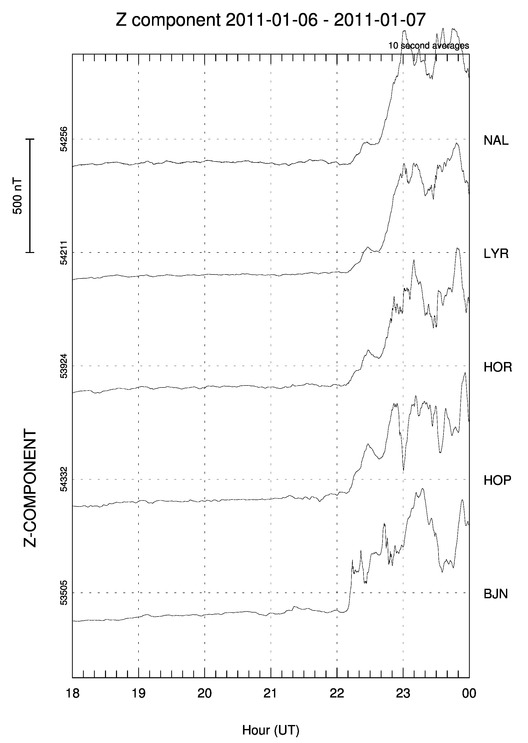
\includegraphics[width=.8\linewidth]{Z_gram.jpg}
		\caption{$B_Z$ at zero altitude for different locations, 18 - 24 UT}
		\label{mag1}
	\end{subfigure}
	\begin{subfigure}[h]{.5\textwidth}
		\centering
		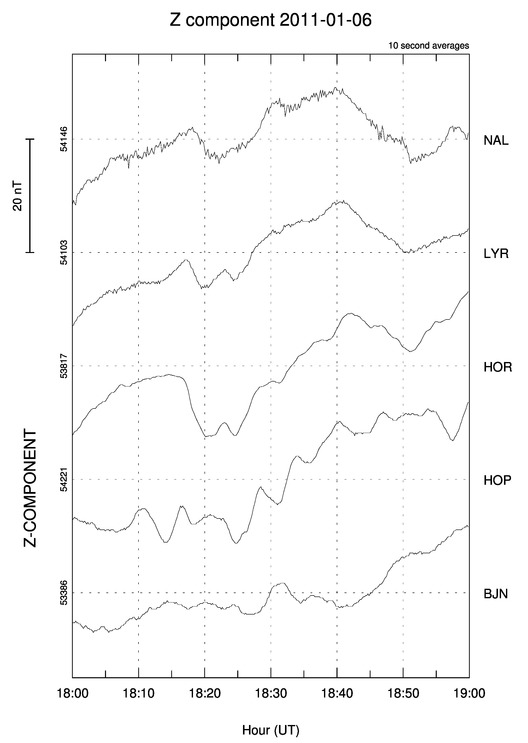
\includegraphics[width=.8\linewidth]{Z_gram1.jpg}
		\caption{$B_Z$ at zero altitude for different locations, 18 - 29 UT}
		\label{mag2}
	\end{subfigure}
	\begin{subfigure}[h]{.5\textwidth}
		\centering
		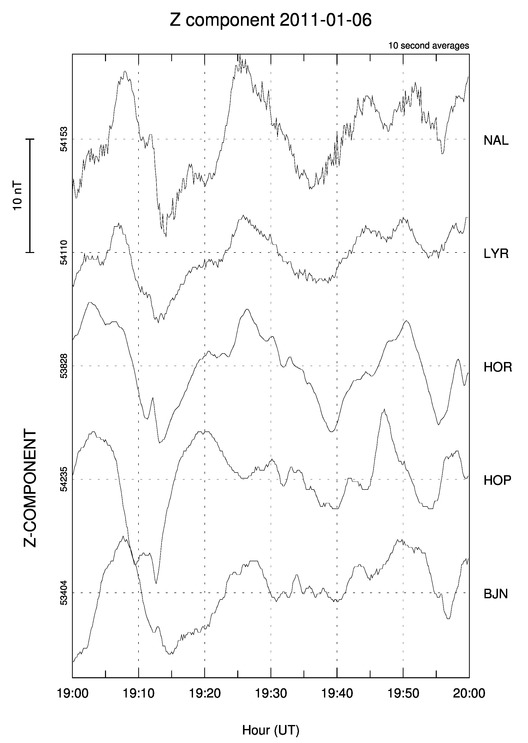
\includegraphics[width=.8\linewidth]{Z_gram2.jpg}
		\caption{$B_Z$ at zero altitude for different locations, 19 - 20 UT}
		\label{mag3}
	\end{subfigure}
	\begin{subfigure}[h]{.5\textwidth}
		\centering
		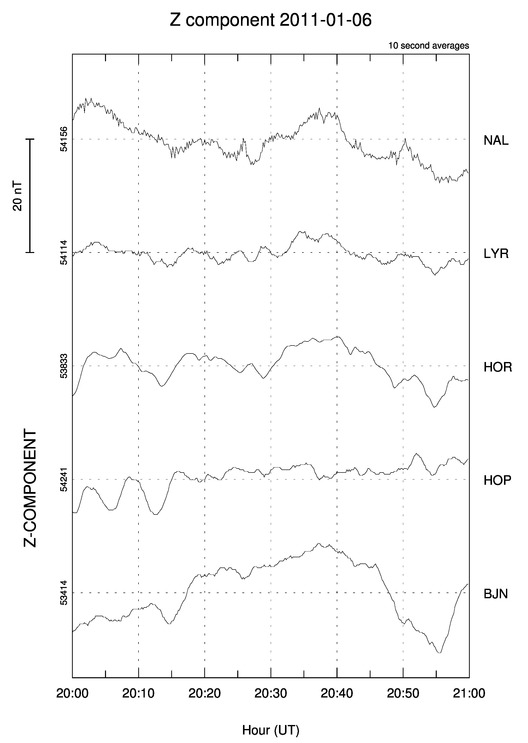
\includegraphics[width=.8\linewidth]{Z_gram3.jpg}
		\caption{$B_Z$ at zero altitude for different locations, 20 - 21 UT}
		\label{mag4}
	\end{subfigure}
	\caption{Measurements of Ground-Based Magnetometers}
	\label{mag}
\end{figure}
\begin{figure}[h]
	\begin{subfigure}[h]{.5\textwidth}
		\centering
		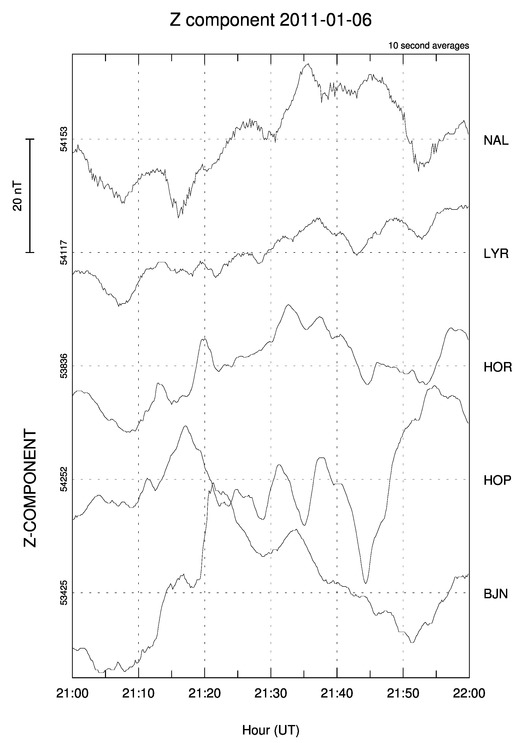
\includegraphics[width=.8\linewidth]{Z_gram4.jpg}
		\caption{$B_Z$ at zero altitude for different locations, 21 - 22 UT}
		\label{mag5}
	\end{subfigure}
	\begin{subfigure}[h]{.5\textwidth}
		\centering
		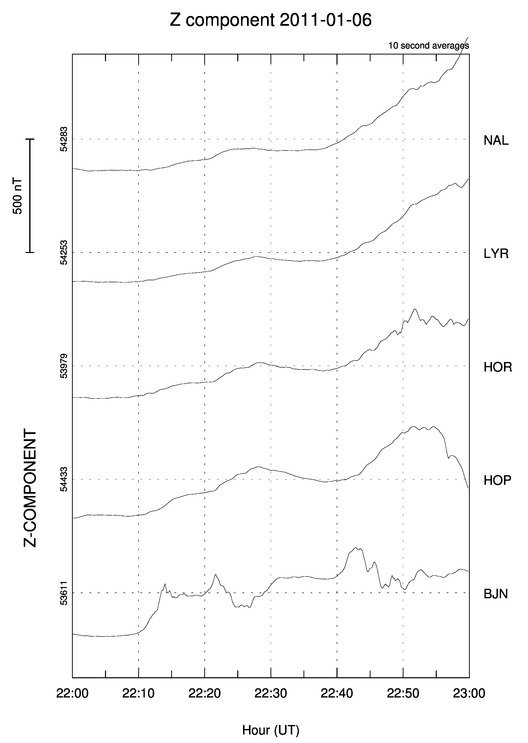
\includegraphics[width=.8\linewidth]{Z_gram5.jpg}
		\caption{$B_Z$ at zero altitude for different locations, 22 - 23 UT}
		\label{mag6}
	\end{subfigure}
	\begin{subfigure}[h]{.5\textwidth}
		\centering
		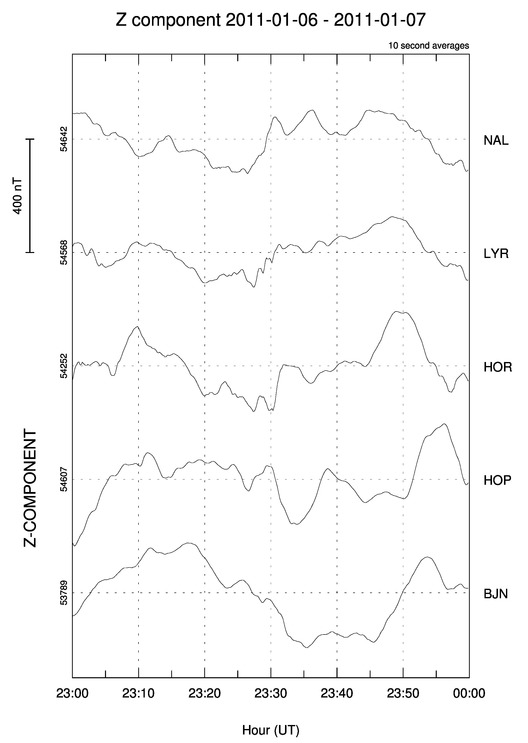
\includegraphics[width=.8\linewidth]{Z_gram6.jpg}
		\caption{$B_Z$ at zero altitude for different locations, 23 - 24 UT}
		\label{mag7}
	\end{subfigure}
	\caption{Measurements of Ground-Based Magnetometers}
	\label{magg}
\end{figure}

\subsection{SuperDARN}

To plot the measurement of the plasma convection in the F-region, and study its velocity and other features that will appear which will be more apparent as the magnetic reconnection happens, we first set the instrument to the Pykkvibaer, located in Iceland and it is directed to the Svalbard area.

First, we look at the polar cap in the interval 17:58 UT-1800 UT. The vectors represent the velocity of the convection, with different colours according to magnitude.

Now it is important to interpret what we see here. The Earth's magnetic field causes the plasma that is settled to flow in a pattern that can be seen from the coloured arrows. Based on these currents, the plot also shows the field potentials, and the equipotential lines with value $\phi$ measured in kV:

The trajectory of the plasma flow can be observed by the arrows, and its possible to have an idea about the velocities.

The aspects we will notice from now on, and try to relate to magnetic reconnection and help to investigate the auroral activity, are the size of the polar cap, the velocity of the plasma flow and the pattern of  the equipotential lines. For 17:58 UT-1800 UT (figure \ref{darn1}), the polar cap size is small, as well as the velocities, where the vectors appear as green and blue. This suggests that reconnection has not happened yet. The potential value is the expected for quiet times, where the average is about 50kV ([1] pg.:303)

If we run the plot approximately one hour later (figure \ref{darn2}), at the magnetometers it can be seen (figure \ref{mag1}), that we have a minimum of magnetic activity around this time. As a consequence $\phi$ must be lower than before. Also the polar cap size has to stay small. As well as the velocity, that might be the same or lower at most regions than at 18 UT. This way, we cannot expect magnetic reconnection.

Looking at the figure, we see that $\phi$ is just $31 kV$, as expected, and also  the velocity is lower, with green and blue arrows dominating (between 250 m/s and few lines around 500 m/s), the distribution of the equipotential lines changed considerably, but this is also expected from «quiet times».

For the next hour(20 UT- 21 UT), it was measured that the solar wind and its IMF get negative at the ACE satellite and at approximately 21:15 UT would be able to interact with the magnetopause through magnetic reconnection. So, for 20 UT - 21 UT, basically the same magnetic activity is expected, with no significant changes in the polar cap size.

At figure \ref{darn3} we can see that at 20 UT, the potential is essentially the same, as well as the velocities, in average, but, the equipotential lines pattern change again, with the polar cap still at the same size. From the magnetometer data, in this time interval, the magnetic field increased, to intervals of $20 nT$, which might have influenced the $E x B$ drift, so the pattern is more similar to the first one, at 18 UT.


At 20 UT - 21 UT, and some minutes after that, the situation stays nearly the same, but by the time that the solar wind was predicted to reach the magnetopause, the equipotential lines change drastically, where the two cell pattern is not as visible as before, and this holds until 21:30 UT, where the pattern returns to something similar as the previous ones. But, we notice that the potential is the lowest with $25kV$, but also the polar cap increases a bit.

However around 21:45 UT, the polar cap increases even more with the potential reaching $51 kV$. At 21:55 UT, we see the polar cap size and the high potential, and also the convection velocity of at least 500 m/s in average (figure \ref{darn5}).

At 22:20 UT, the auroral activity, seen at the All-sky camera, begins (figure \ref{darn6}). We should expect a high velocity convection as well as high $\phi$ beginning with this time, but our observed potential is still low. Only around 10 minutes later, we see that the velocity increases considerably.  And additional 14 minutes later (figure \ref{darn7}), the pattern is essentially what we will see until around 24 UT.

One of the maximum values for the potential and also for the velocities, where in some regions, it is  around 1000 m/s, happens at 22:48-22:50 UT (figure \ref{darn8}), with a potential measured at $79 kV$, and the polar cap size is the largest of the pictures shown.


\begin{figure}[h]
	\begin{subfigure}[h]{.5\textwidth}
		\centering
		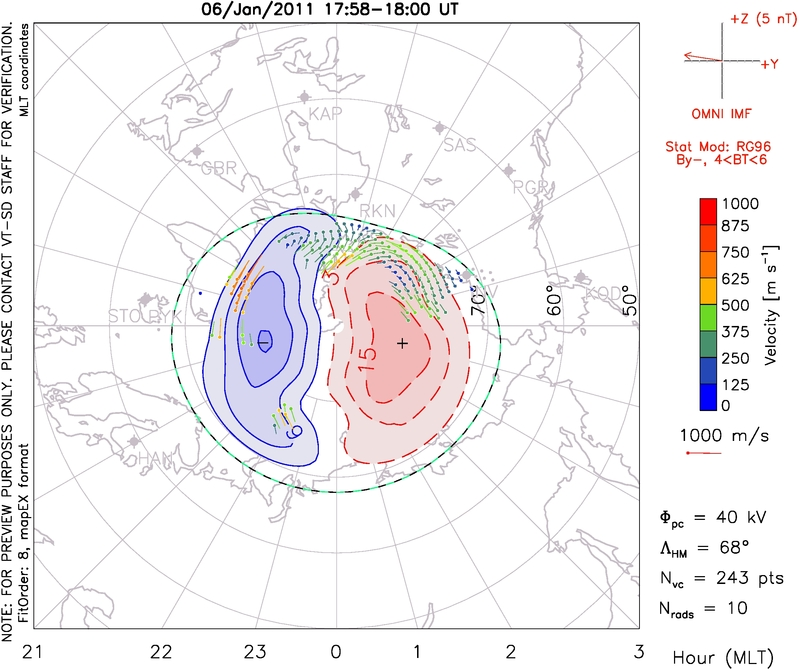
\includegraphics[width=.8\linewidth]{pot_1449158247.jpg}
		\caption{Plasma convection at the northern polar cap, 17:58 - 18:00 UT}
		\label{darn1}
	\end{subfigure}
	\begin{subfigure}[h]{.5\textwidth}
		\centering
		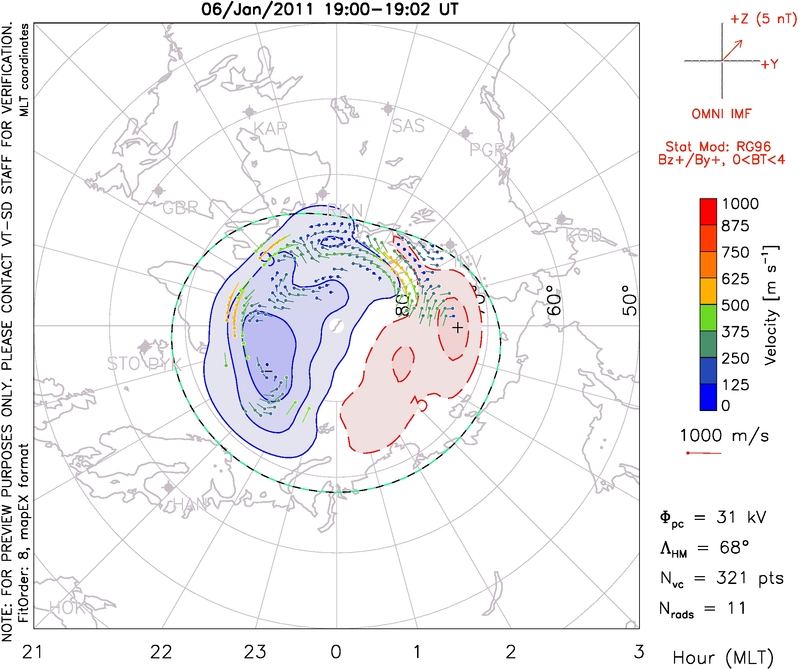
\includegraphics[width=.8\linewidth]{pot_1449158282.jpg}
		\caption{Plasma convection at the northern polar cap, 19:00 - 19:02 UT}
		\label{darn2}
	\end{subfigure}
	\begin{subfigure}[h]{.5\textwidth}
		\centering
		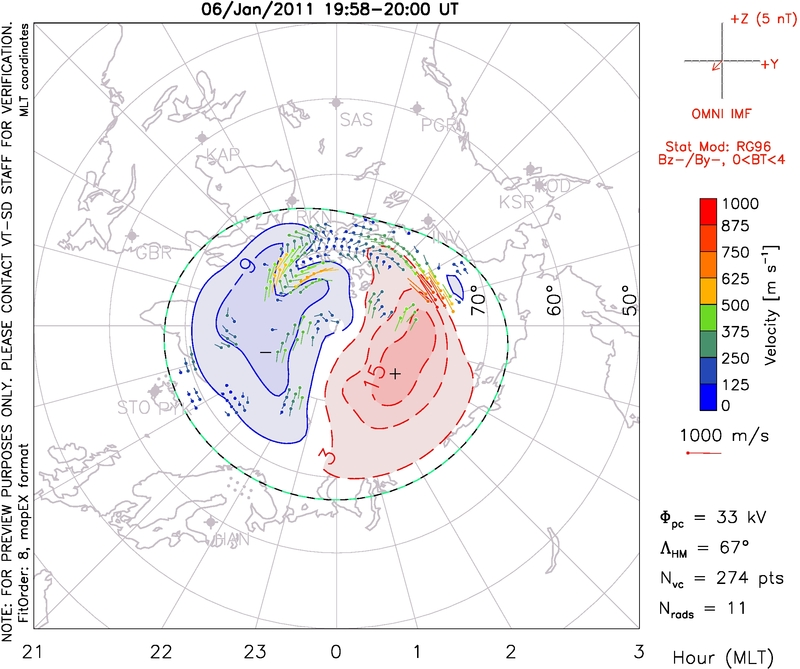
\includegraphics[width=.8\linewidth]{pot_1449158312.jpg}
		\caption{Plasma convection at the northern polar cap, 19:58 - 20:00 UT}
		\label{darn3}
	\end{subfigure}
	\begin{subfigure}[h]{.5\textwidth}
		\centering
		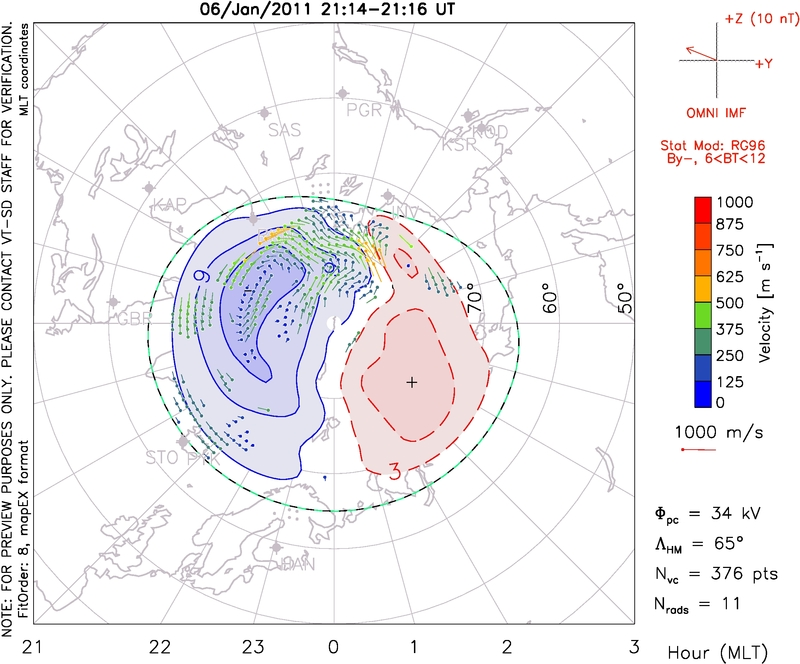
\includegraphics[width=.8\linewidth]{pot_1449158341.jpg}
		\caption{Plasma convection at the northern polar cap, 21:14 - 21:16 UT}
		\label{darn4}
	\end{subfigure}
	\begin{subfigure}[h]{.5\textwidth}
		\centering
		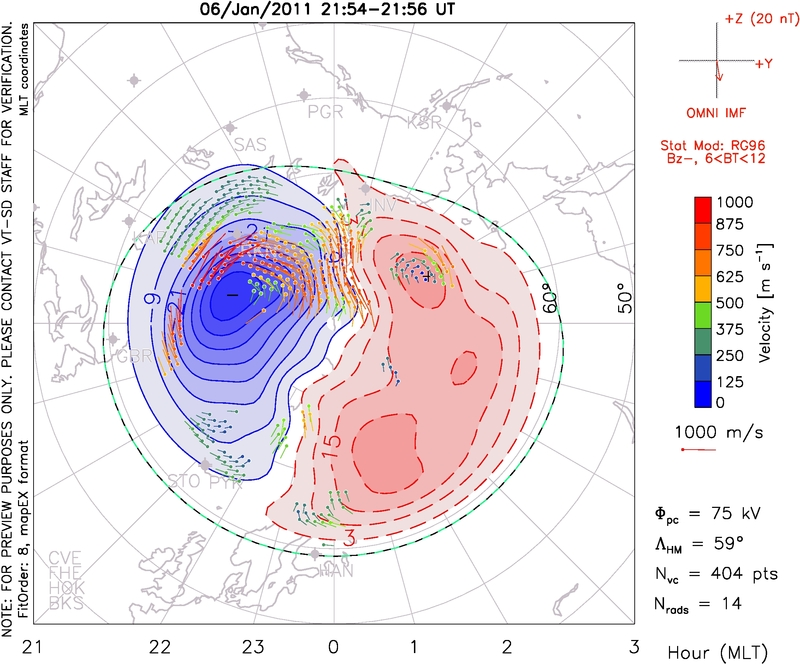
\includegraphics[width=.8\linewidth]{pot_1449158369.jpg}
		\caption{Plasma convection at the northern polar cap, 21:54 - 21:56 UT}
		\label{darn5}
	\end{subfigure}
\begin{subfigure}[h]{.5\textwidth}
	\centering
	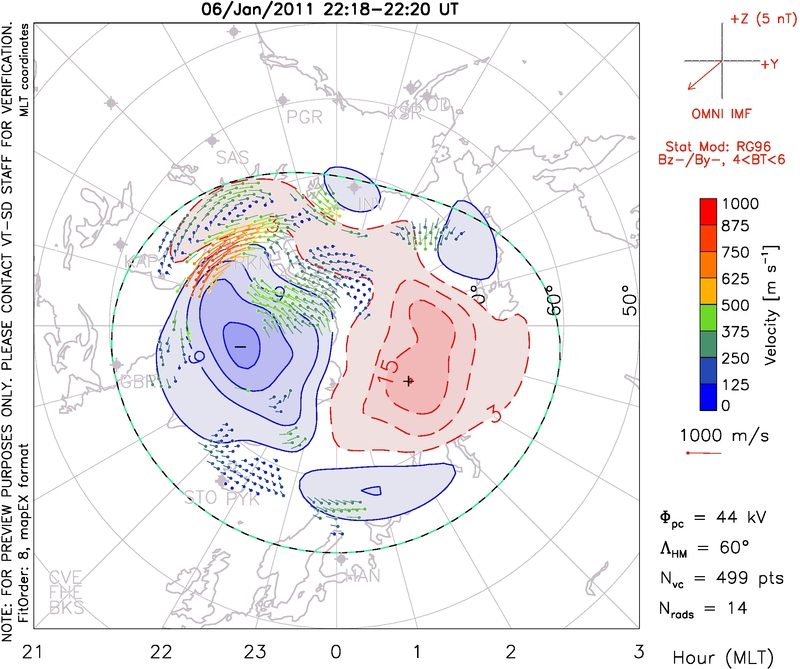
\includegraphics[width=.8\linewidth]{pot_1449166790.jpg}
	\caption{Plasma convection at the northern polar cap, 22:18 - 22:20 UT}
	\label{darn6}
\end{subfigure}
\begin{subfigure}[h]{.5\textwidth}
	\centering
	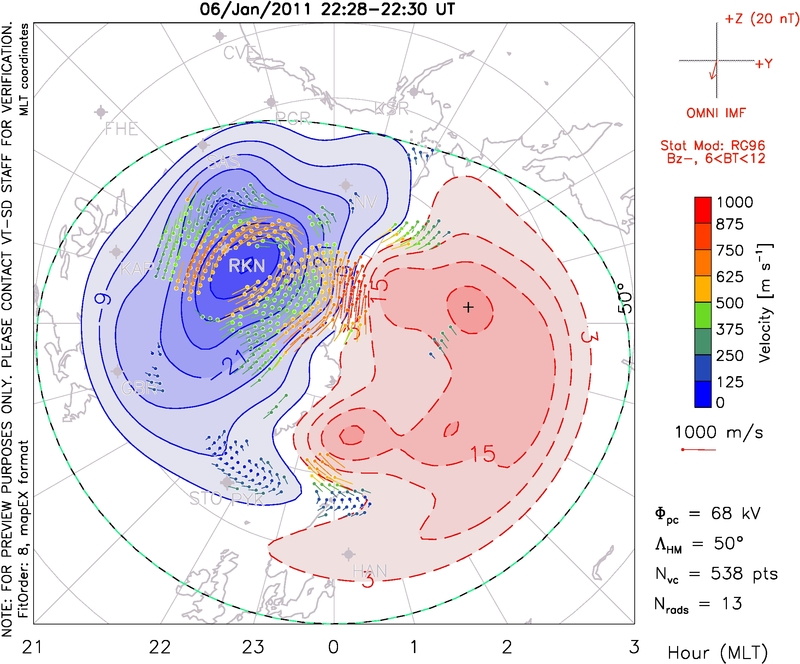
\includegraphics[width=.8\linewidth]{pot_1449173054.jpg}
	\caption{Plasma convection at the northern polar cap, 22:28 - 22:30 UT}
	\label{darn9}
\end{subfigure}
\begin{subfigure}[h]{.5\textwidth}
	\centering
	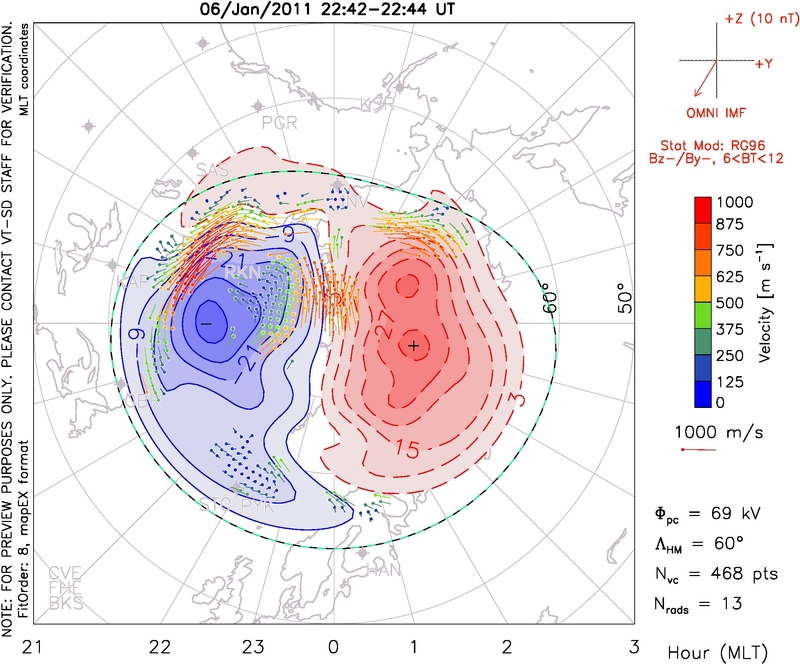
\includegraphics[width=.8\linewidth]{pot_1449167770.jpg}
	\caption{Plasma convection at the northern polar cap, 22:42 - 22:44 UT}
	\label{darn7}
\end{subfigure}
	\caption{Measurements of the SuperDARN}
	\label{darn}
\end{figure}

\begin{figure}[h]
\begin{subfigure}[h]{.5\textwidth}
	\centering
	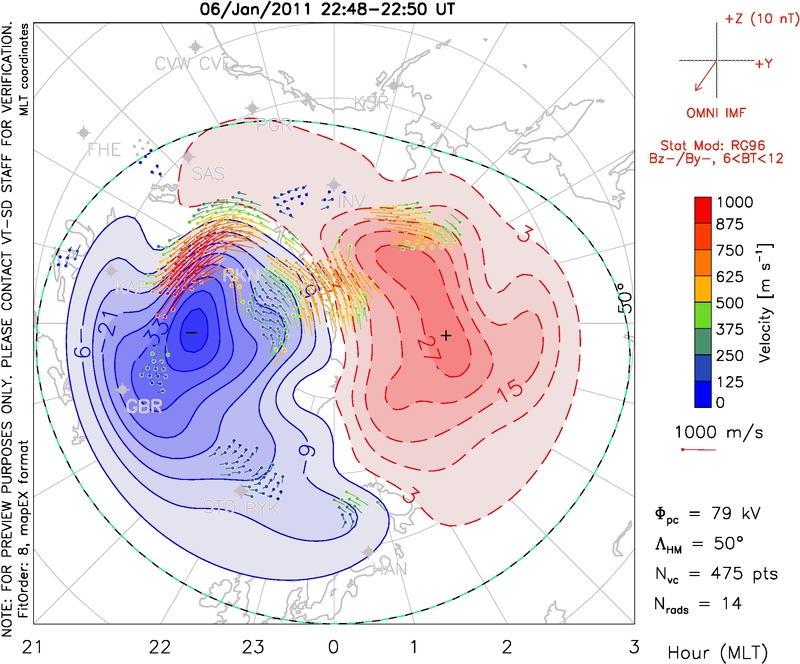
\includegraphics[width=.8\linewidth]{pot_1449168502.jpg}
	\caption{Plasma convection at the northern polar cap, 22:48 - 22:50 UT}
	\label{darn8}
\end{subfigure}
\begin{subfigure}[h]{.5\textwidth}
	\centering
	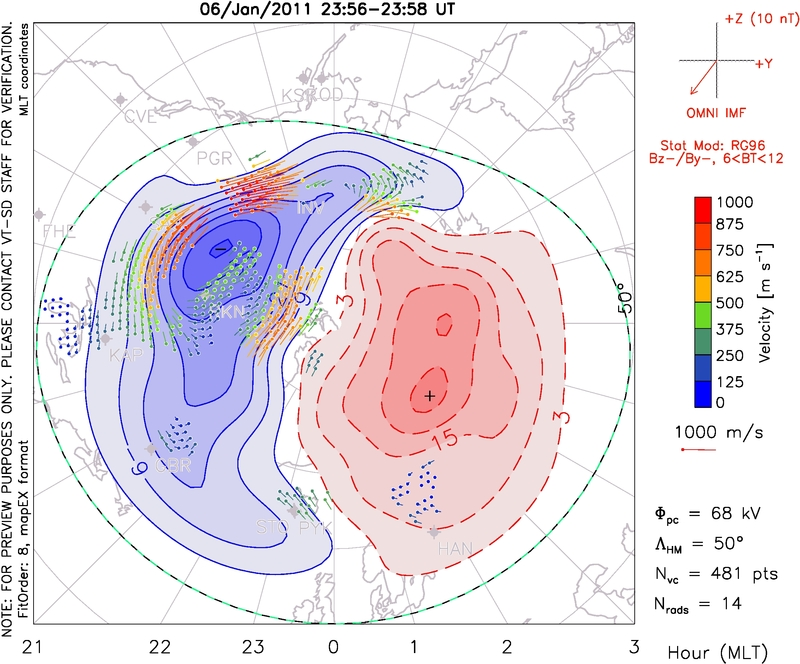
\includegraphics[width=.8\linewidth]{pot_1449173267.jpg}
	\caption{Plasma convection at the northern polar cap, 23:56 - 23:58 UT}
	\label{darn10}
\end{subfigure}

\caption{Measurements of the SuperDARN}
\label{darnn}
\end{figure}

\section{Discussion}

At the 6. January 2011 between 18 UT and 24 UT a substorm was happening at earth. This storm can be seen in the data of the instruments we observed.
While mostly having a northward component the time before 21:15 UT, the z-component of the solar wind at the magnetopause changes sign at this time such that magnetic reconnection becomes possible.

Before that time, the field-aligned currents of Earth are not intense and there are few variations. Also there is little plasma convection in the ionosphere, where the electric potential observed, is the predicted for quiet times ($50 kV$), which are the times when there is no magnetic reconnection. Also the magnetic field measured at ground at the polar cap is almost constant, which means that there is not much current activity in the ionosphere. When we get a southward IMF at around 21:15 UT, the magnetic field  frozen-in to the solar wind interacts with the Earth's magnetic field for longer times, this frozen-in concept is broken and these lines are reconnected, and this is reflected in the data we analysed.

We also notice that the in the ionosphere, before at low velocities, once magnetic reconnection is possible, the convections increases. Due to dayside reconnection the polar cap increases in size. It is the biggest around 22:30 UT. The due to the solar wind magnetic reconnected field lines and the plasma ,frozen-in in them, get pulled to the night side and the Dungey-cycle gets executed. This leads to, due to the frozen-in plasma, more convection happening in the polar cap (figure \ref{darn5}).
The bigger amound of convection also produces an electric potential which has during the night the maximum value at around 79kV (figure \ref{darn5}). Hence the current system of the ionosphere and magnetosphere increases and more current is flowing (figure \ref{amp4}, \ref{mag1}).

The auroral activity due to the beginning of the expansion phase of the sub storm can first be seen at 22:45 UT, when particles on the magnetic field lines, which reconnected at the near-earth neutral-line, move down the field lines with high energy. The consequences of those particles is a sudden onset of aurora which at 23:28 UT already covers nearly the hole sky, the All-sky camera observes (figure \ref{i2}). Due to the sudden magnetic reconnection on the nightside, the polar cap decreases in size quickly, such that the auroras travel northward up to over 80° MLAT.

Du to the nightside reconnection of the expansion phase of the substorm, the size of the polar cap decreases (figure \ref{darn7}). The reconnected field lines and their frozen-in plasma travel to the dayside and cause a lot of convection in the ionosphere (figure \ref{darn7}), which causes an increasing electric potential. Due to this, the magnitude of the current system in the ionosphere increase. Beginning with the start of the expansion phase the Birkeland currents are increased a lot (figures \ref*{amp5},\ref*{amp6}, \ref*{amp7}) and the strong currents cause disturbances in the magnetic field, measured at the ground at the polar cap (\ref{mag1}). Even at 24 UT the substorm has not ended.


\section{Sources}


	\url{http://tid.uio.no/plasma/aurora/tech.html}
	
	\url{https://en.wikipedia.org/wiki/Advanced_Composition_Explorer}
	
	\url{https://en.wikipedia.org/wiki/Super_Dual_Auroral_Radar_Network}
	
	\url{https://en.wikipedia.org/wiki/Iridium_satellite_constellation}
	
	\url{http://www.jhuapl.edu/newscenter/pressreleases/2010/100818.asp}
	
	\url{https://directory.eoportal.org/web/eoportal/satellite-missions/a/ampere}

	\url{http://tid.uio.no/plasma/aurora/data.php}
	
	\url{http://vt.superdarn.org/tiki-index.php?page=radarFoV}
	
	\url{http://space.fmi.fi/image/beta/?page=real_time#}
	
	\url{http://ampere.jhuapl.edu/}
	
	\url{http://cdaweb.gsfc.nasa.gov/cdaweb/istp_public/}
	
\section{Graphics}


\end{document}